\documentclass[a4paper]{article}

%% Language and font encodings
\usepackage[english]{babel}
\usepackage[utf8x]{inputenc}
\usepackage[T1]{fontenc}
\usepackage{amsmath}

%% Sets page size and margins
\usepackage[a4paper,top=3cm,bottom=2cm,left=3cm,right=3cm,marginparwidth=1.75cm]{geometry}

%% Useful packages
\usepackage{amsmath}
\usepackage{amsthm}
\usepackage{amssymb}
\usepackage{graphicx}
\usepackage[colorinlistoftodos]{todonotes}
\usepackage[colorlinks=true, allcolors=blue]{hyperref}
\usepackage{neuralnetwork}
\usepackage{sidecap}

\newtheorem{theorem}{Theorem}[section]
\newtheorem{corollary}{Corollary}[theorem]
\newtheorem{lemma}[theorem]{Lemma}

\newcommand{\setreal}{\mathbb{R}}

\title{Cheatsheet for Fisher-Rao Metric, Geometry, and Complexity of Neural Networks}
\author{Sandro Braun, Leander Kurscheidt}

\begin{document}
\maketitle
\begin{abstract}
\end{abstract}
\section{Geometry of Deep Rectified Networks}


\subsection{Lemma 2.1}

\begin{lemma}[Structure in Gradients]
	\begin{align}
		\label{lemma_structure_in_gradient}
		\sum_{t=0}^{L} \sum_{i \in [k_t], j \in [k_{t+1}]} \frac{\partial O^{L+1}}{\partial W^{t_{ij}}} W^t_{ij} = (L+1)O^{L+1}(x) = \langle \nabla_\theta f_\theta (x), \theta \rangle
	\end{align}
\end{lemma}

\subsubsection{Example for Lemma 2.1}

\begin{minipage}{.5\textwidth}
	\begin{neuralnetwork}[height=2]
		\newcommand{\nodetextx}[2]{$x_#2$}
		\newcommand{\nodetexty}[2]{$y_#2$}
		\inputlayer[count=2, bias=false, title=$O^0$, text=\nodetextx]
		\outputlayer[count=1, title=$O^1$, text=\nodetexty] \linklayers
	\end{neuralnetwork}
\end{minipage}

Take a simple feed forward neural network with only two inputs and one output. Remember that by definition $O^0 = x$. The simple example can then be written with

\begin{align}
	\label{eq_simple_nn}
	O^0 = 	\begin{bmatrix}
				O^0_1 \\ 
				O^0_2
			\end{bmatrix} &,
	W^0 = 	\begin{bmatrix}
				W^0_1 \\
				W^0_2
			\end{bmatrix} \\
			O^1 &= \sigma({O^0}^T W^0) = \sigma(
											\underbrace{O^0_1 W^0_1 + O^0_2 W^0_2}_z
											).
\end{align}
Substituting the term in brackets will simplify notation.

%\begin{minipage}{.5\textwidth}
Now calculate the partial derivatives of \eqref{eq_simple_nn} with respect to $W^0_i$.
\begin{align*}
	\frac{\partial O^1}{\partial W^0_1} &= \sigma'(z) O^0_1 \\
	\frac{\partial O^1}{\partial W^0_2} &= \sigma'(z) O^0_2
\end{align*}
Summing up the $\frac{\partial O^1}{\partial W_j} W_j$ reveals,

\begin{align*}
	\sum_{j=1}^{2} \frac{\partial O^1}{\partial W^0_j} W^0_j &= \sigma'(z) O^0_1  W^0_1 + \sigma'(z) O^0_2  W^0_2 = \sigma'(z)(\underbrace{O^0_1 W^0_1 + O^0_2 W^0_2}_\text{z}) \\
														&= \sigma'(z) z
\end{align*}
Note that this is equivalent to calculating $\langle \nabla_{W^0} O^1, W^0 \rangle$:
\begin{align*}
	\nabla_{W^0} O^1 &= 
		\begin{bmatrix}
			\frac{\partial O^1}{\partial W^0_1} \\ 
			\frac{\partial O^1}{\partial W^0_2}
		\end{bmatrix} \\
	\langle \nabla_{W^0} O^1, W^0 \rangle &= \sum_{j=1}^{2} \frac{\partial O^1}{\partial W^0_j} W^0_j = \dots = \sigma'(z) z
\end{align*}
Using the relation $\sigma(z) = \sigma'(z)(z)$ reveals \eqref{eq_simple_nn}. Then reading left to right reveals \eqref{lemma_structure_in_gradient} for $L=0$, $\theta= W^0$ and $f_\theta(x) = O^1(x)$ which completes the example.

\begin{align*}
		\sum_{t=0}^{L=0} \sum_{j=1}^{2} \frac{\partial O^1}{\partial W^t_j} W^t_j
		=  \langle \nabla_{W^0} O^1, W^0 \rangle
		= \sigma'(z) z 
		= \sigma(z) = O^1
\end{align*}

%\end{minipage}%


\subsection{Corollary 2.1}

\subsubsection{Notes}
\begin{enumerate}
	\item 
	\begin{proof}
		We want to show $\frac{\partial l(f,Y)}{\partial f} = -y \Leftrightarrow yf < 1$. So,
		\begin{alignat*}{2}
			                && 1-y_if_i &> 0 \\
			\Leftrightarrow && l &=1-y_if_i \\
			\Leftrightarrow && \frac{\partial l}{\partial f} &=-y_i
		\end{alignat*}
	  \end{proof}
	\item 
	\begin{proof}
		We want to show $\frac{\partial l(f,Y)}{\partial f} = 0 \Leftrightarrow yf > 1$. So,
		\begin{alignat*}{2}
							&& 1-y_if_i &< 0 \\
			\Leftrightarrow && l &=0 \\
			\Leftrightarrow && \frac{\partial l}{\partial f} &=0
		\end{alignat*}
	  \end{proof}
\end{enumerate}


\begin{figure}
	\centering
	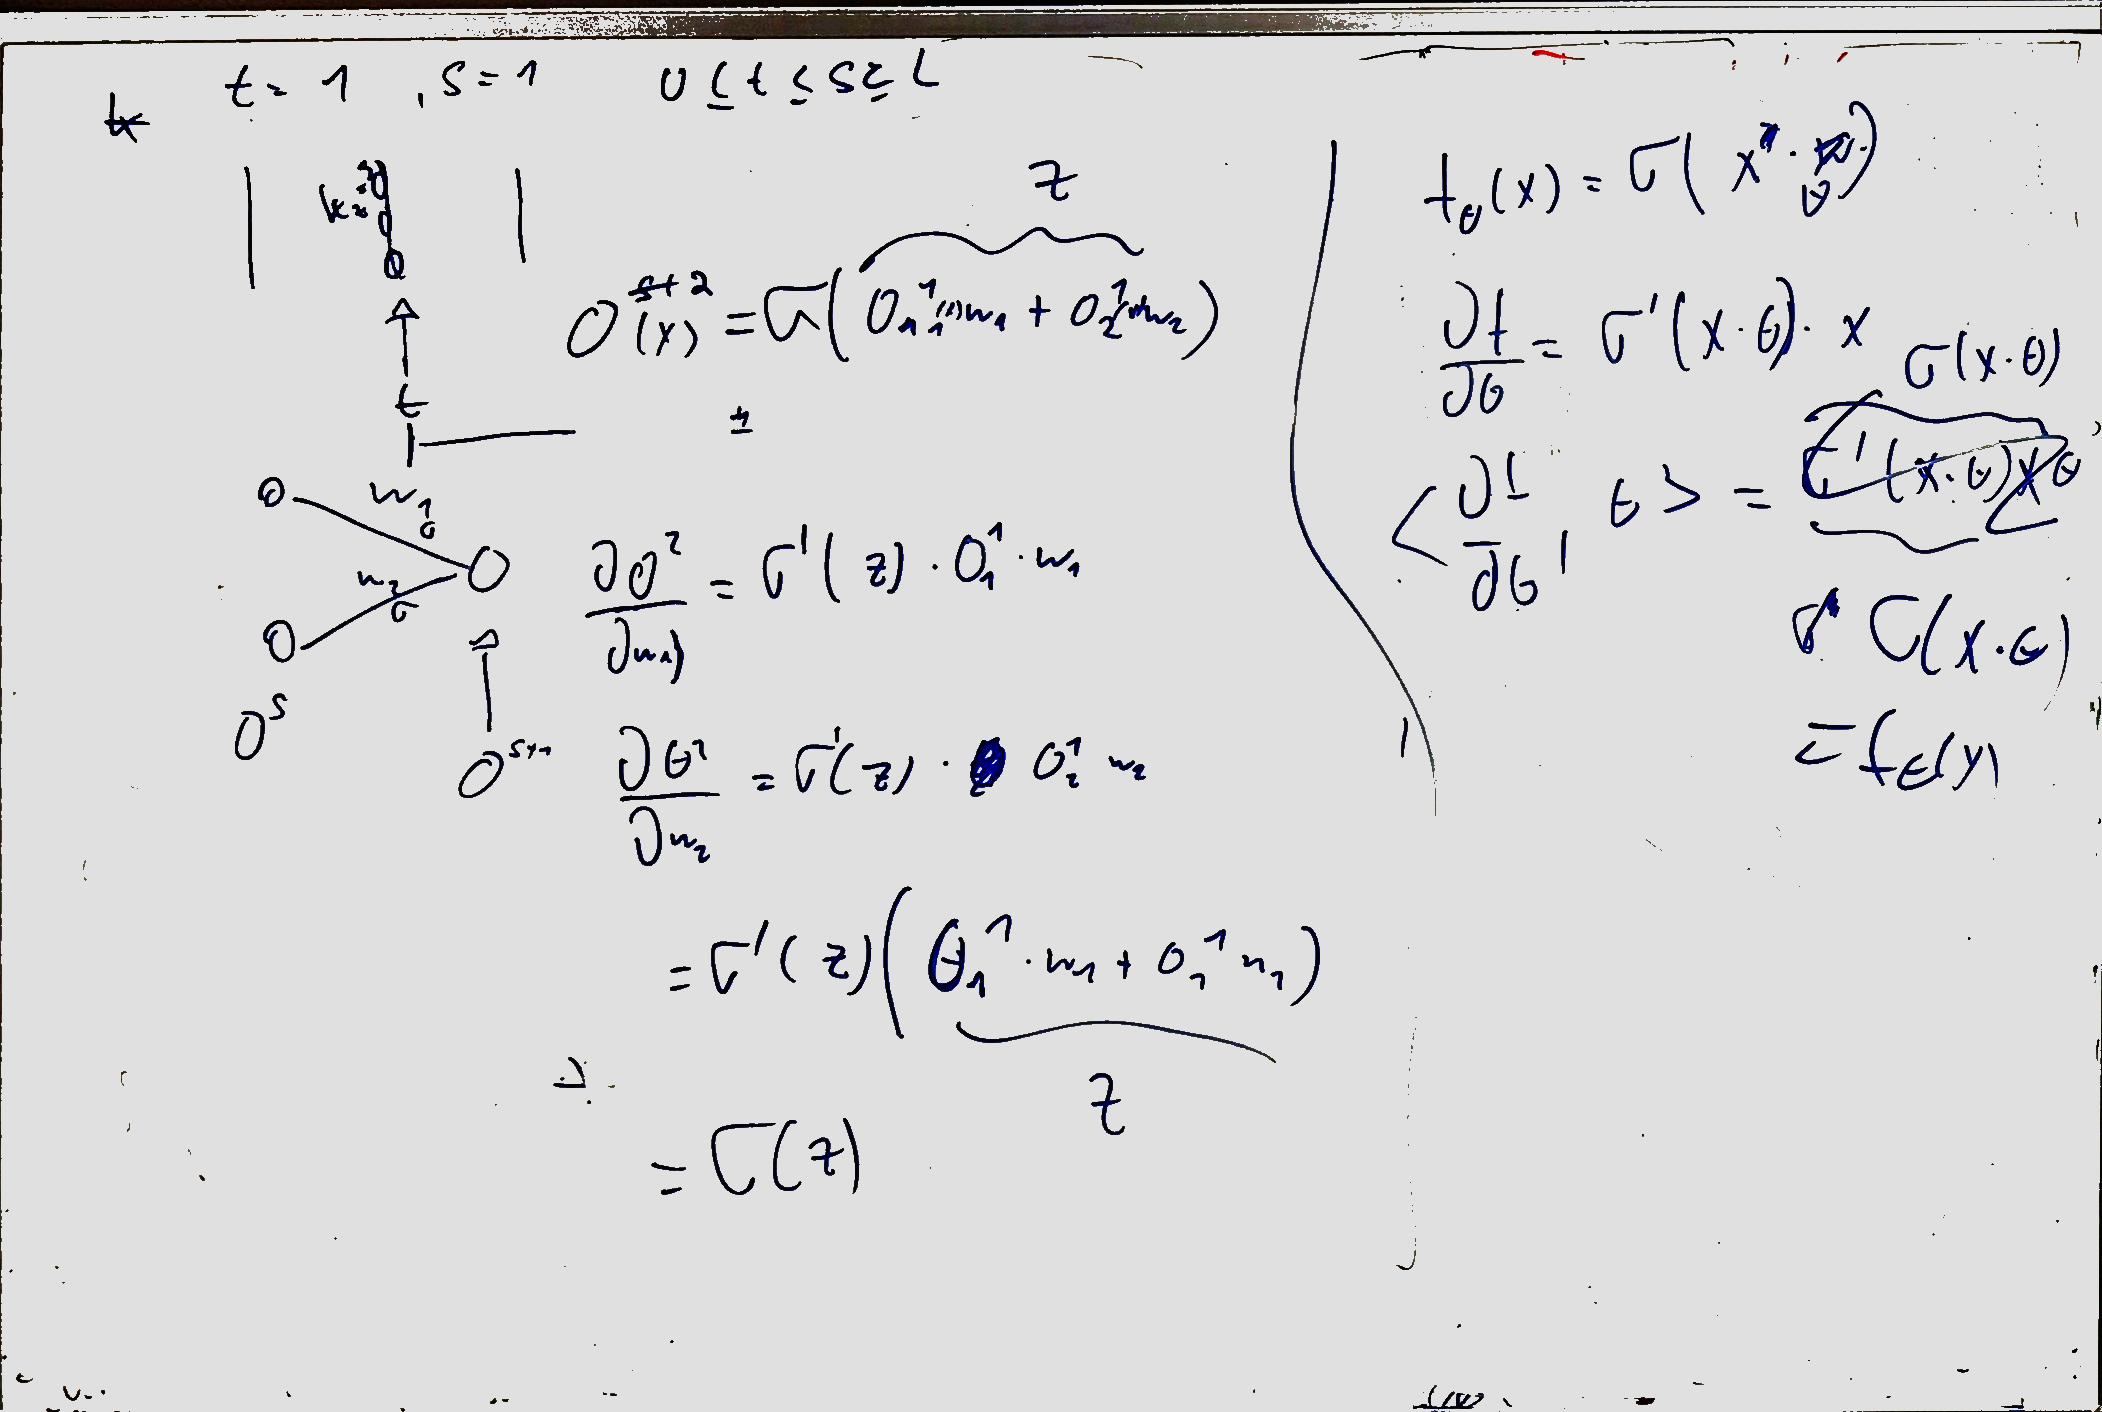
\includegraphics[width=\textwidth]{whiteboard_notes/20180706_01.jpg}
\end{figure}

\begin{figure}
	\centering
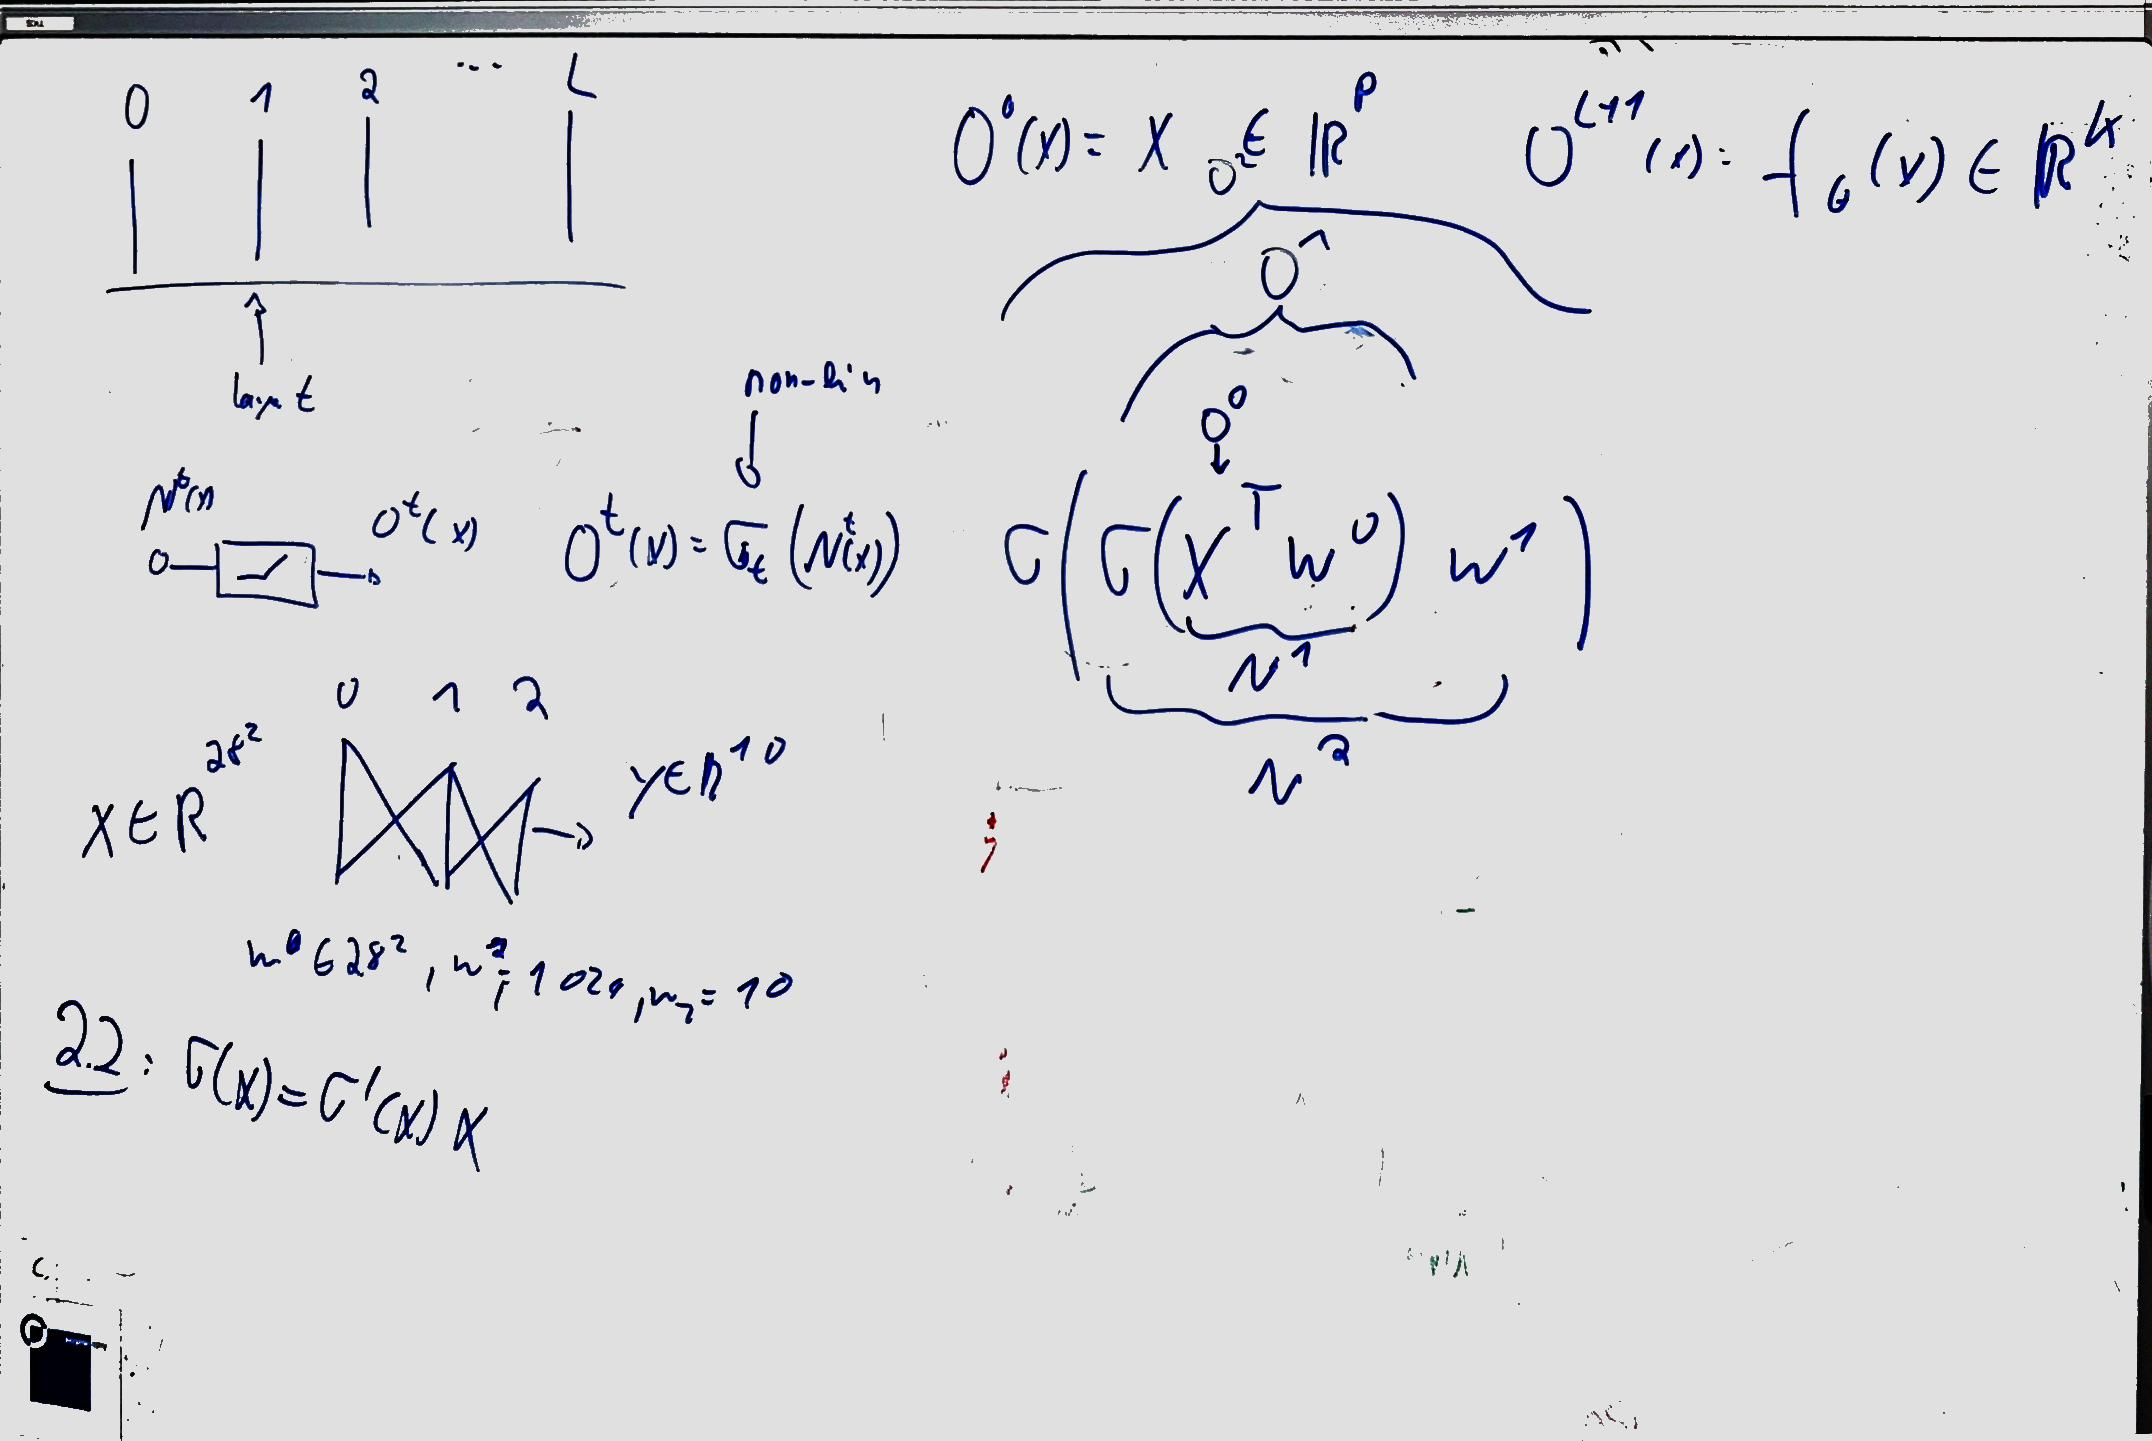
\includegraphics[width=\textwidth]{whiteboard_notes/20180706_02.jpg}
\end{figure}
\begin{figure}
	\centering
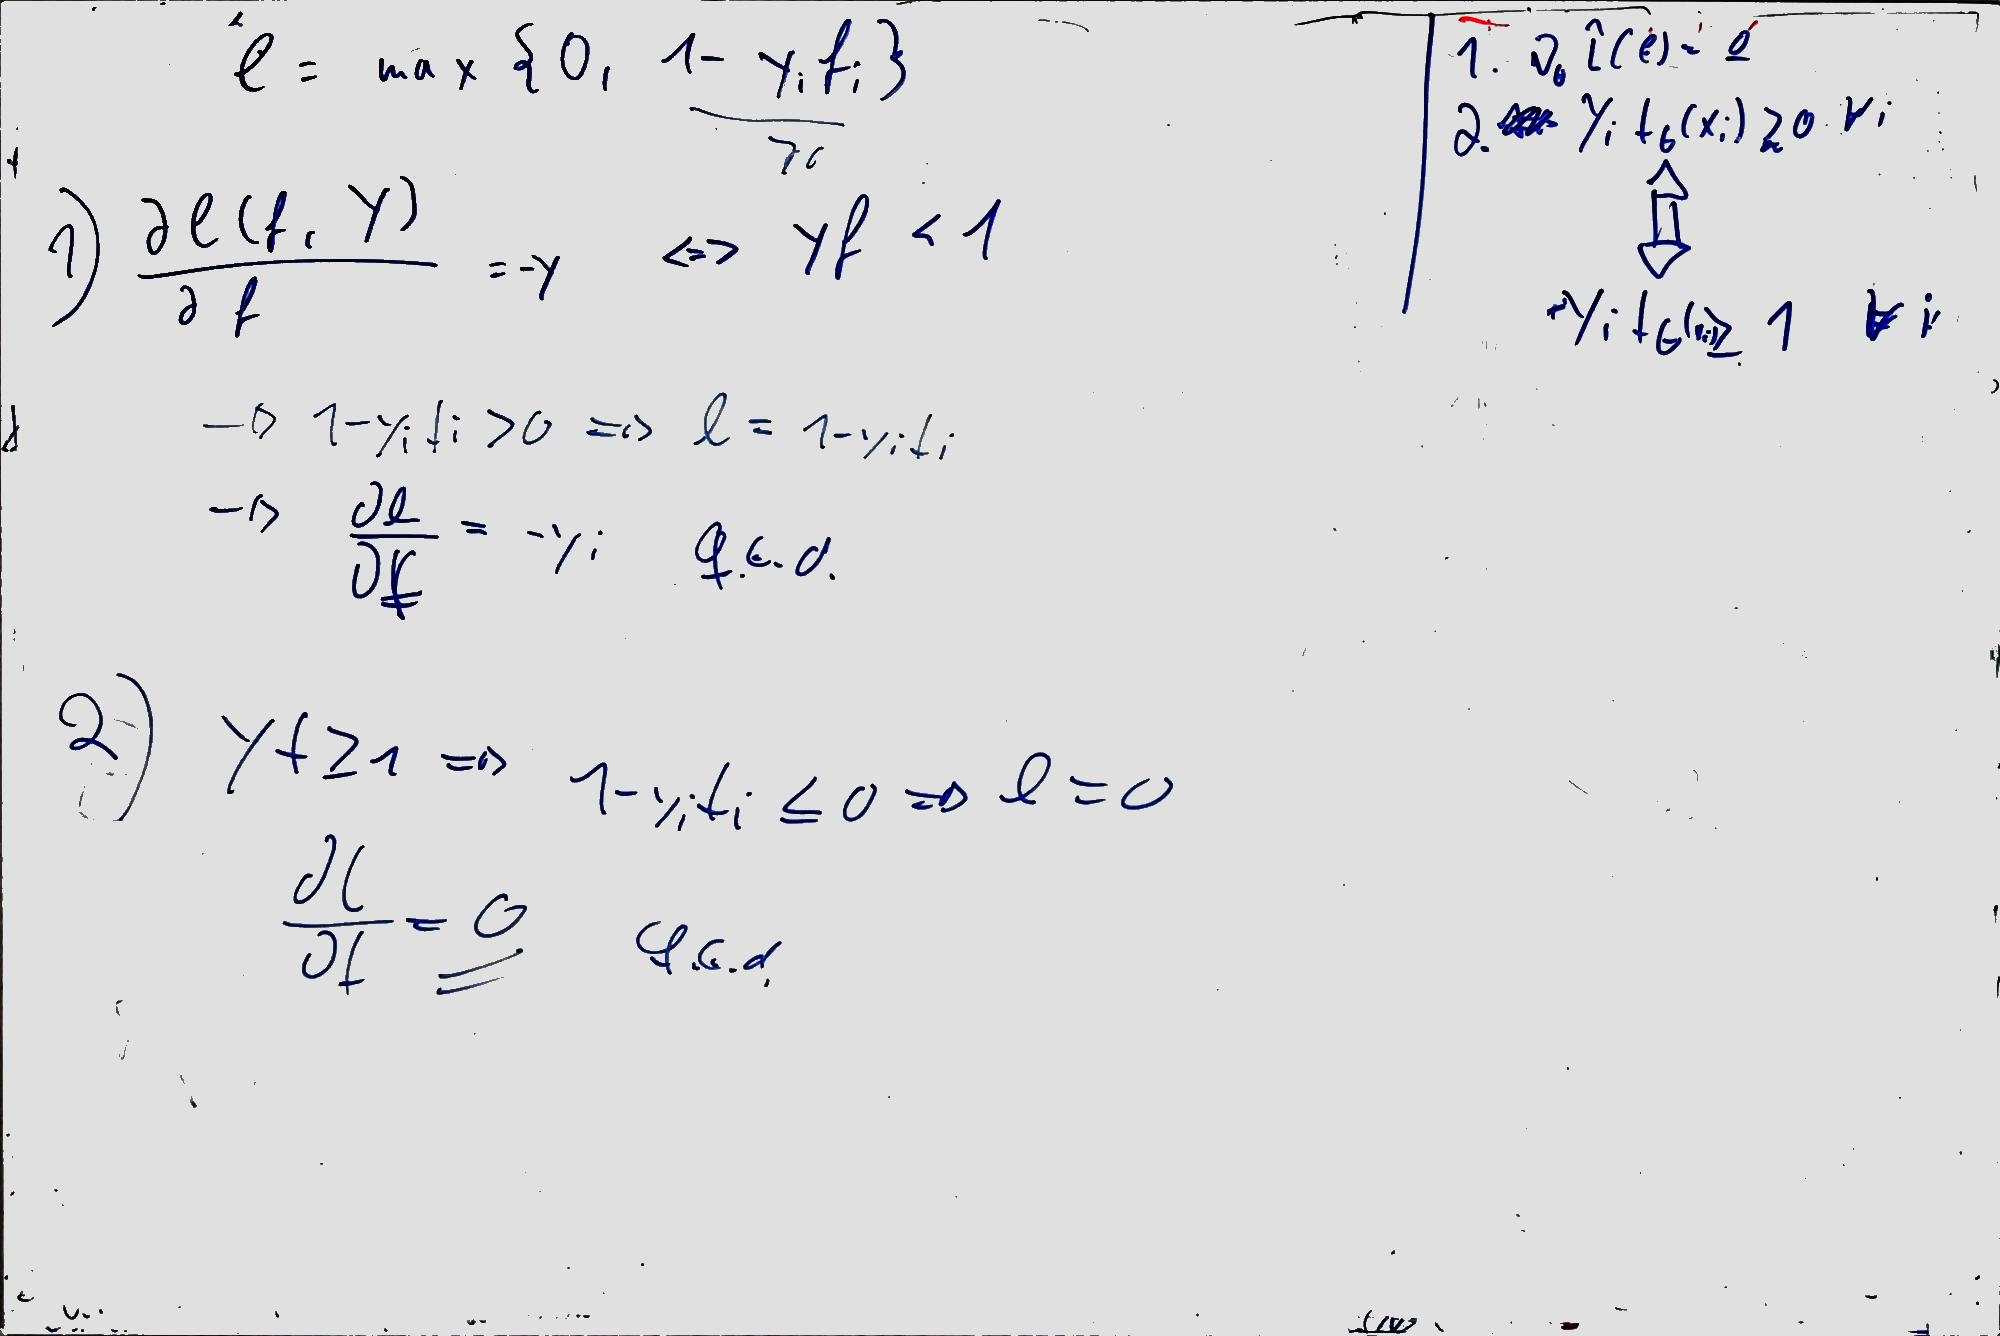
\includegraphics[width=\textwidth]{whiteboard_notes/20180706_03.jpg}
\end{figure}
\begin{figure}
	\centering
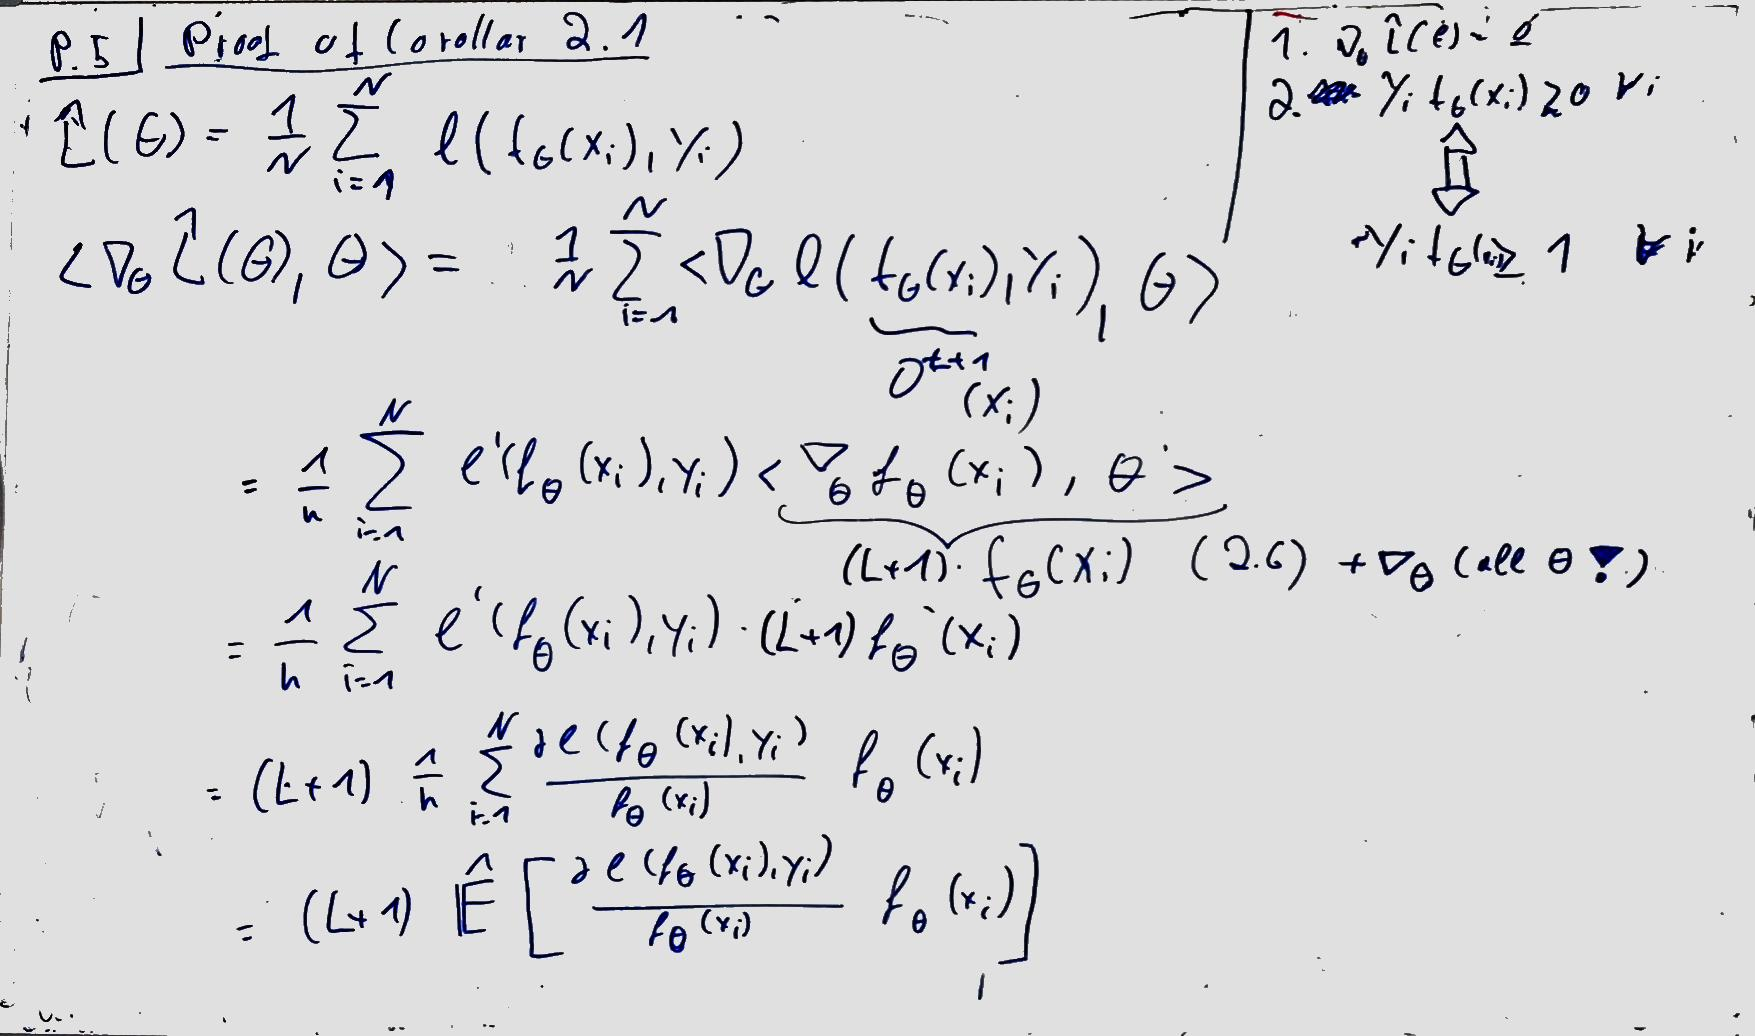
\includegraphics[width=\textwidth]{whiteboard_notes/20180706_04.jpg}
\end{figure}
\begin{figure}
	\centering
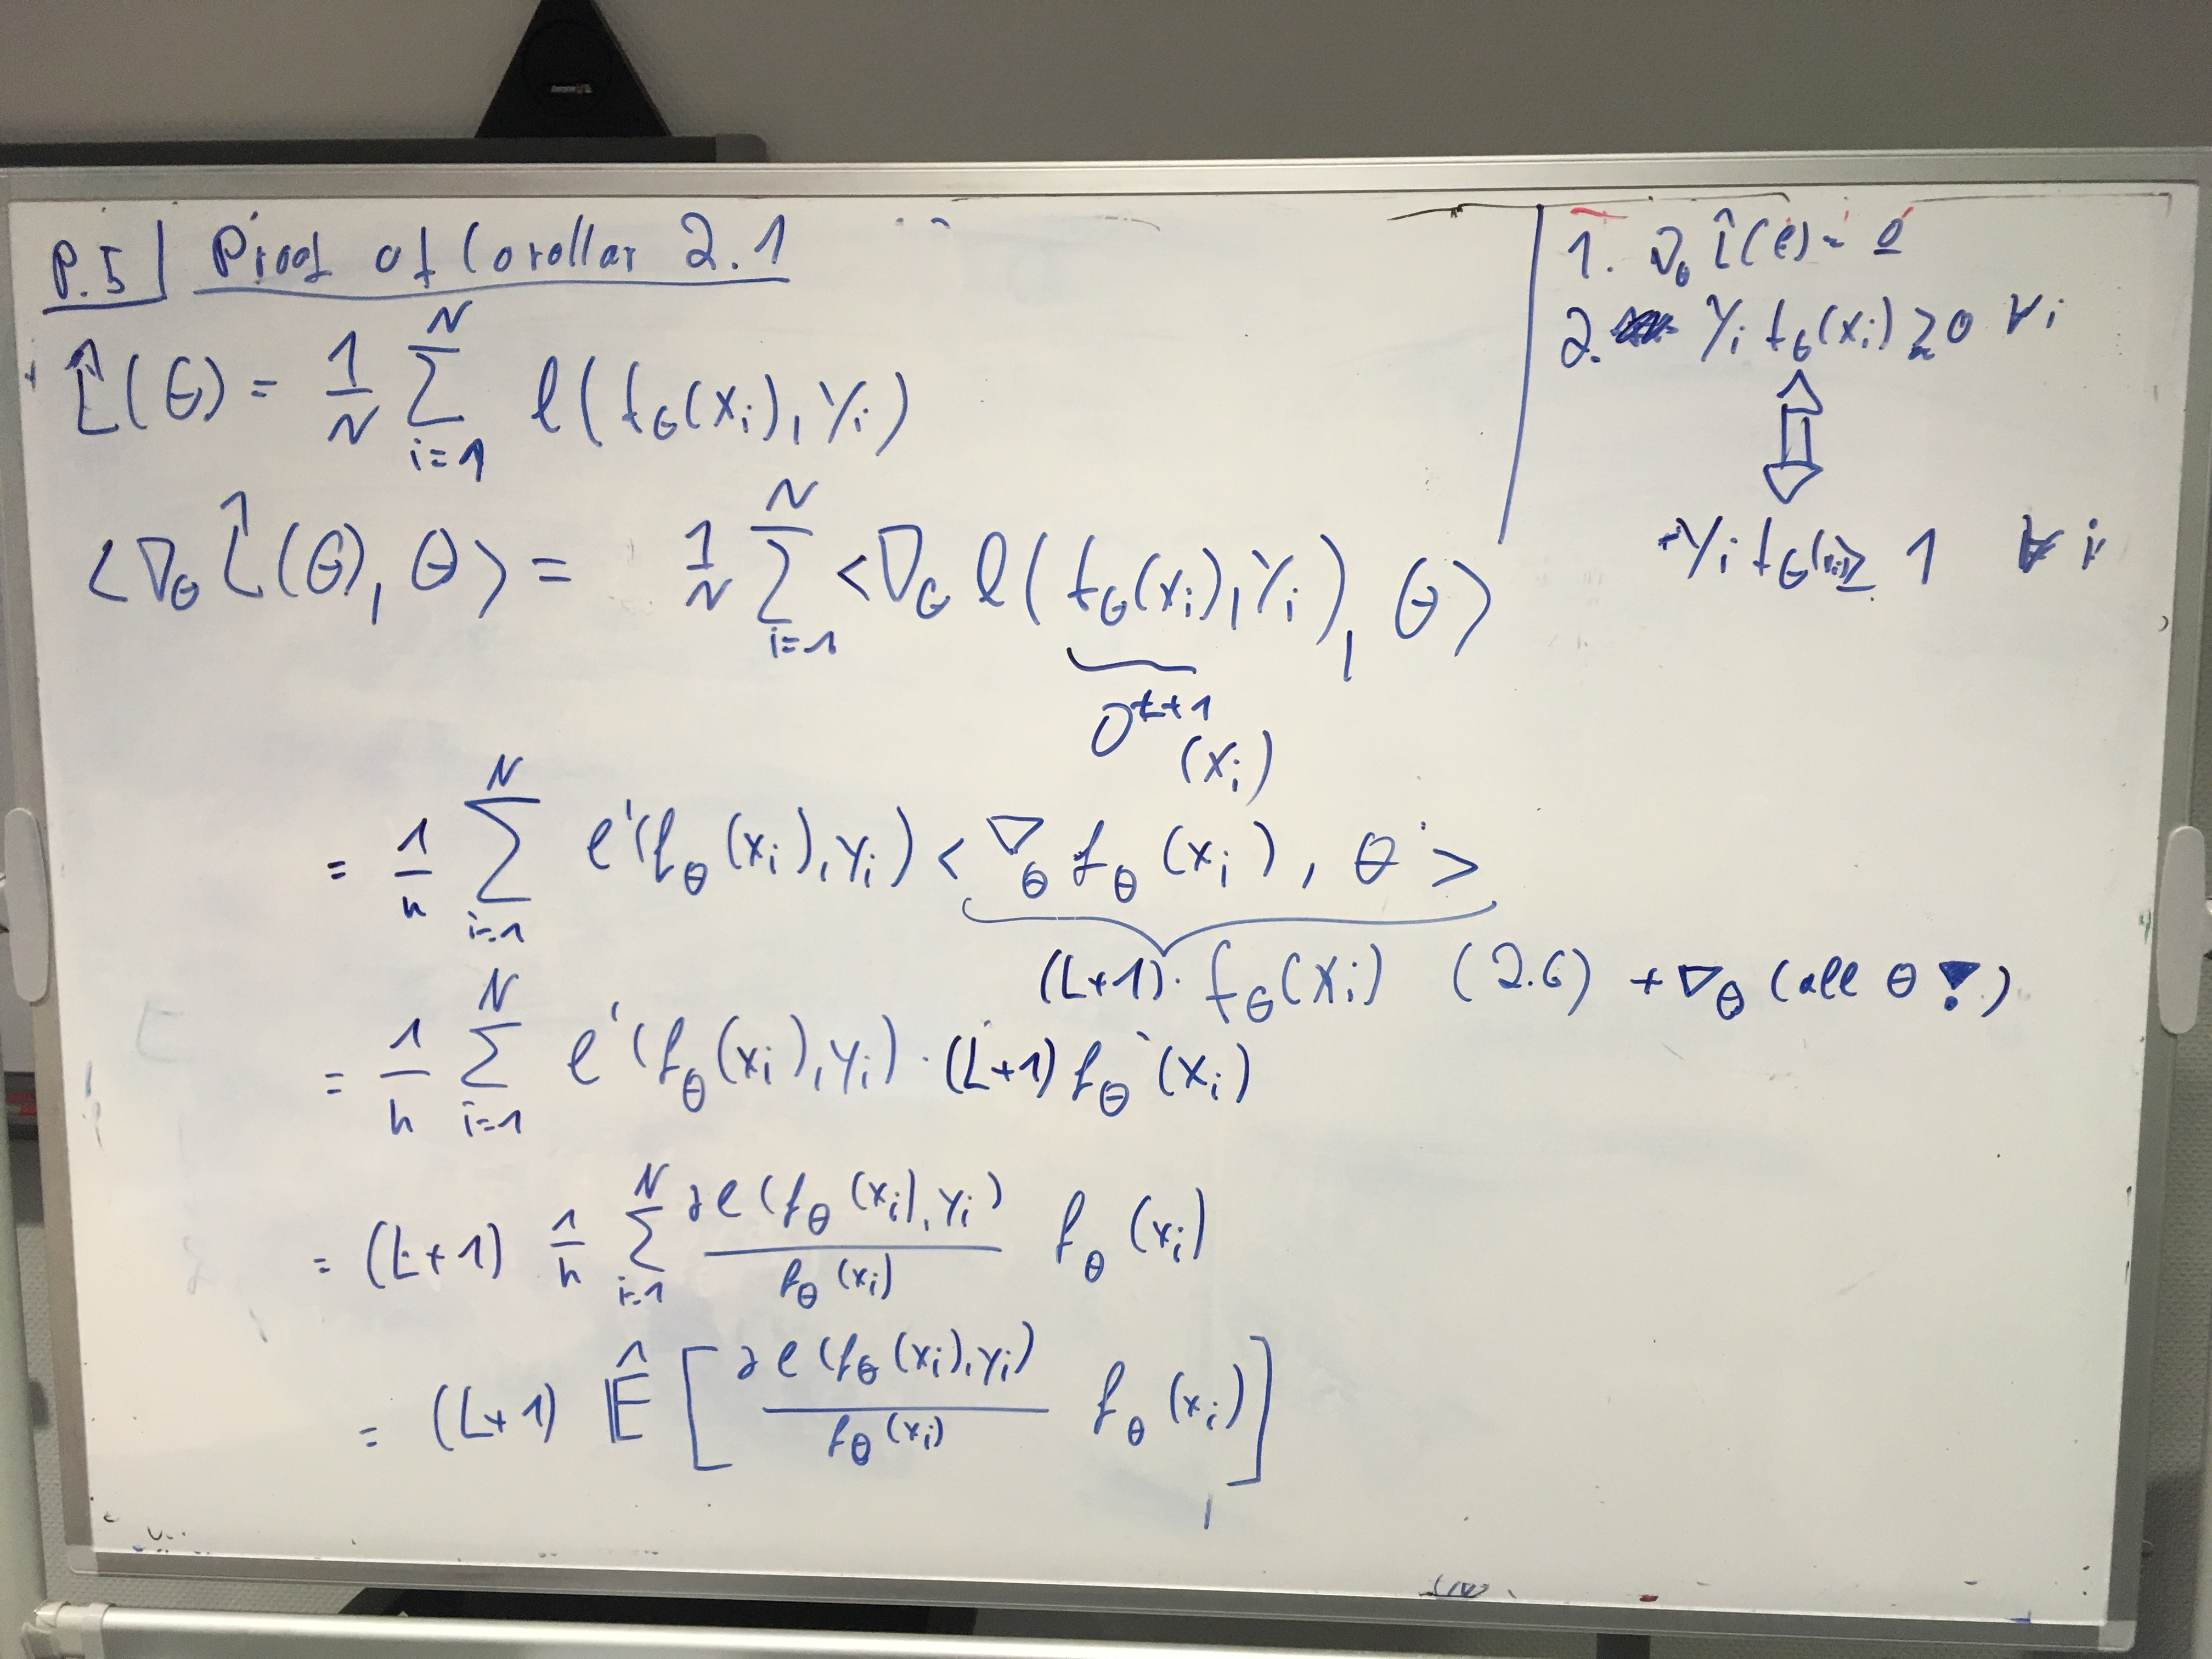
\includegraphics[width=\textwidth]{whiteboard_notes/IMG_1583.jpg}
\end{figure}
\begin{figure}
	\centering
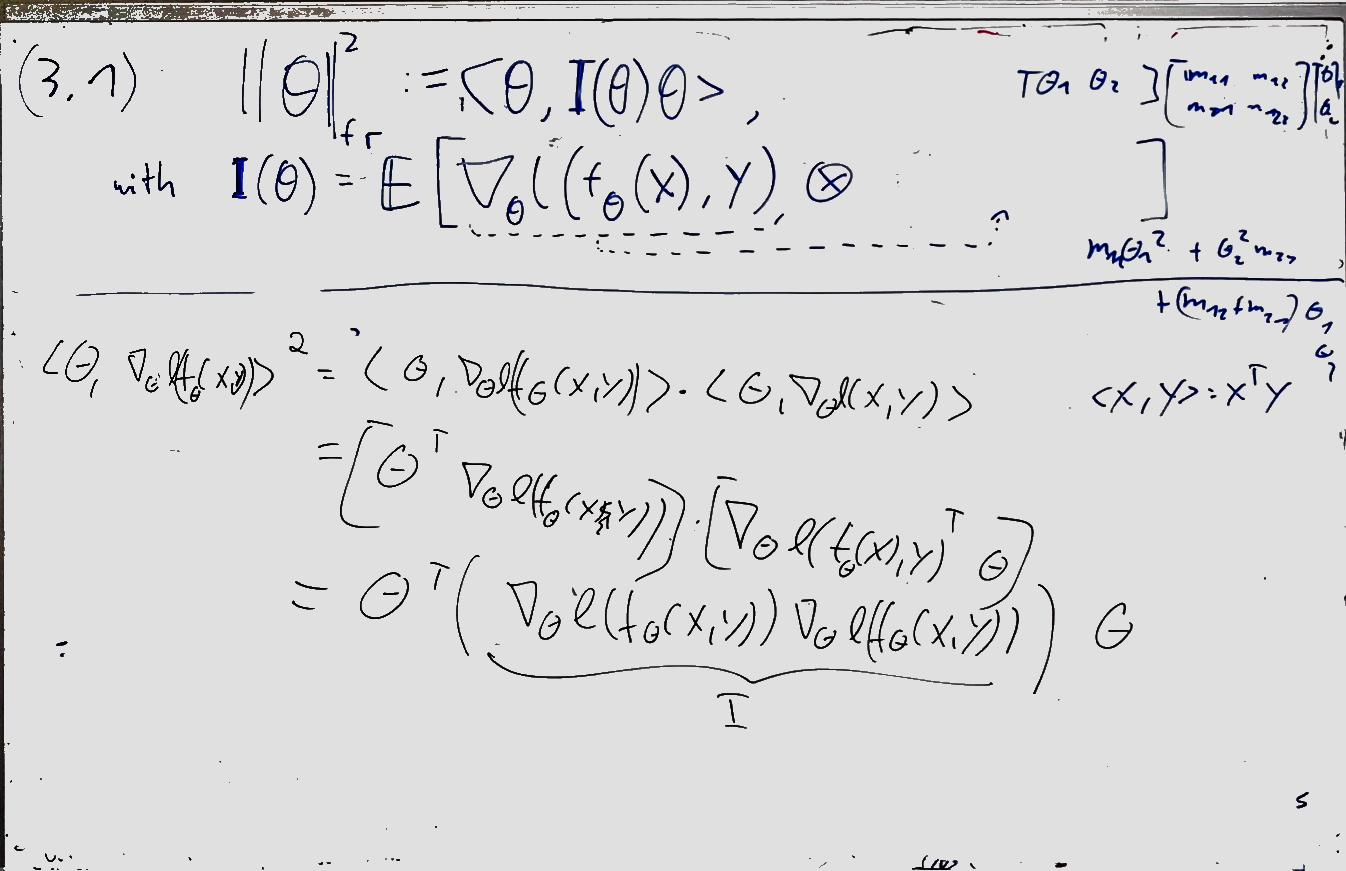
\includegraphics[width=\textwidth]{whiteboard_notes/3_1_proof.jpg}
\end{figure}
\begin{figure}
	\centering
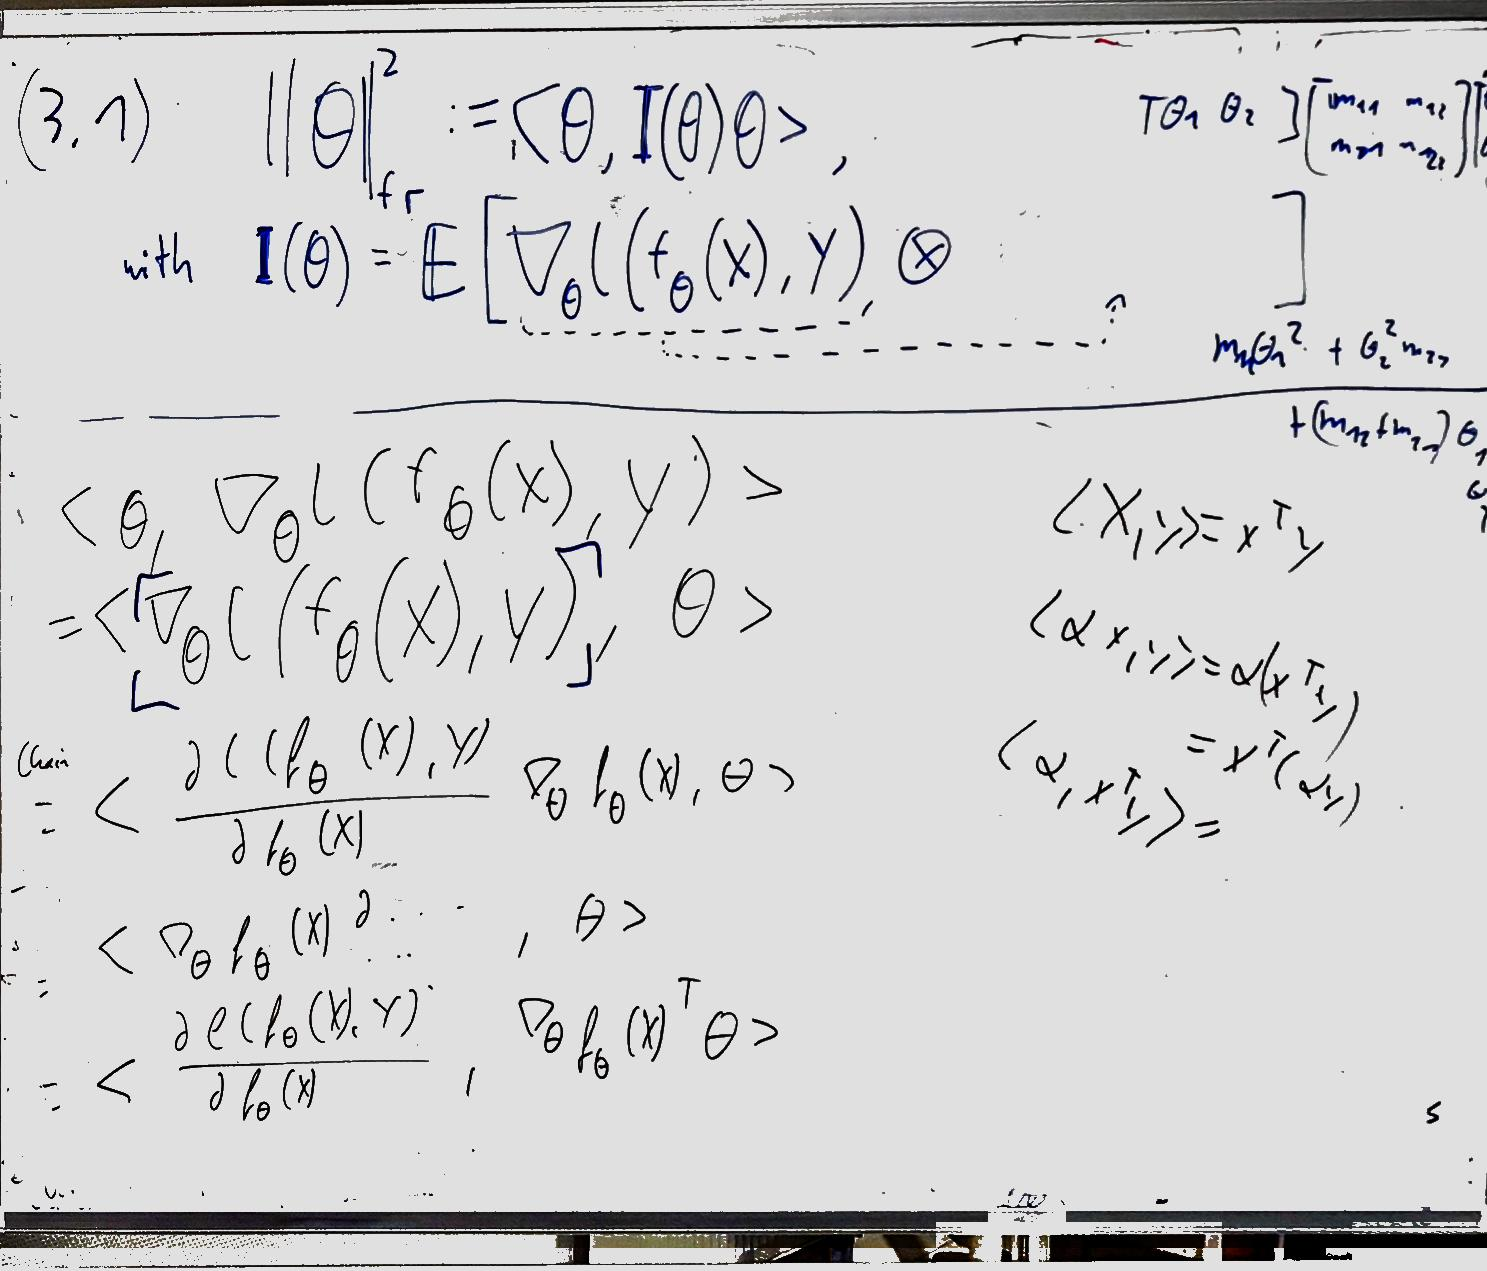
\includegraphics[width=\textwidth]{whiteboard_notes/3_1_proof_cont.jpg}
\end{figure}
\begin{figure}
	\centering
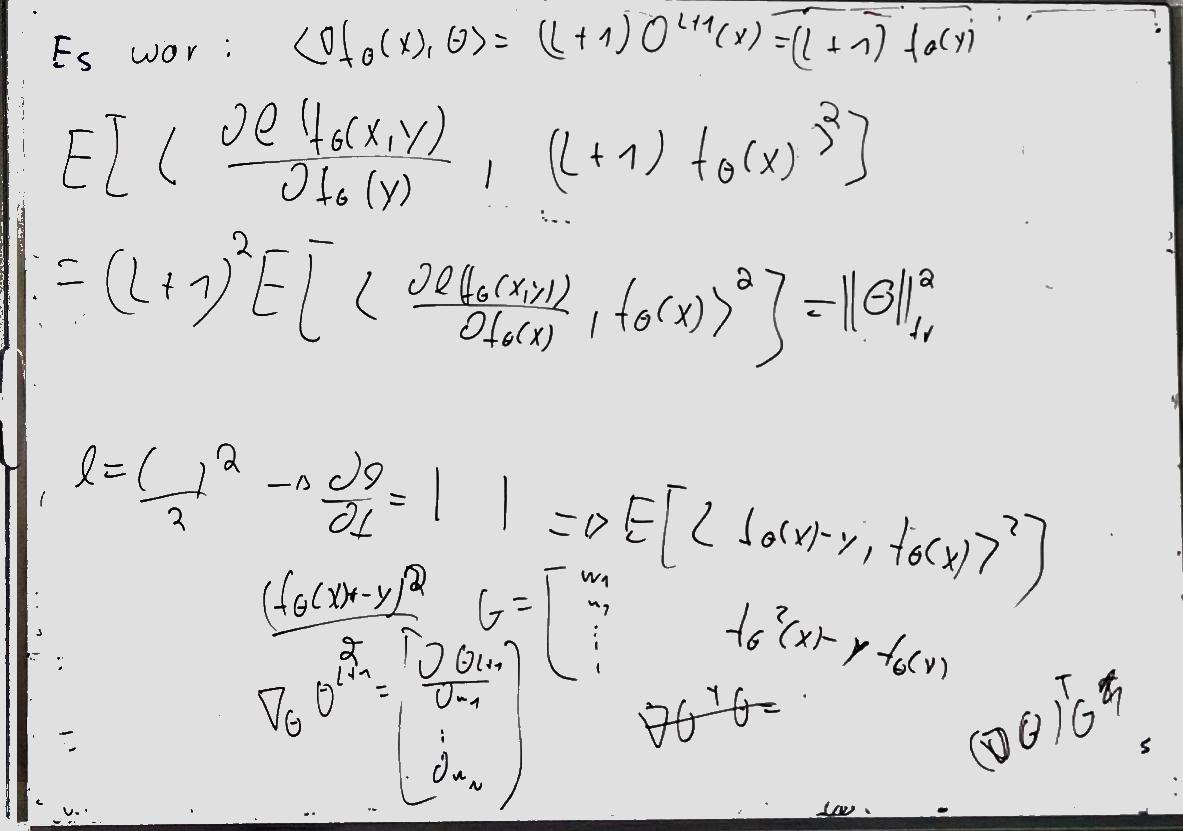
\includegraphics[width=\textwidth]{whiteboard_notes/07.jpg}
\end{figure}
\begin{figure}
	\centering
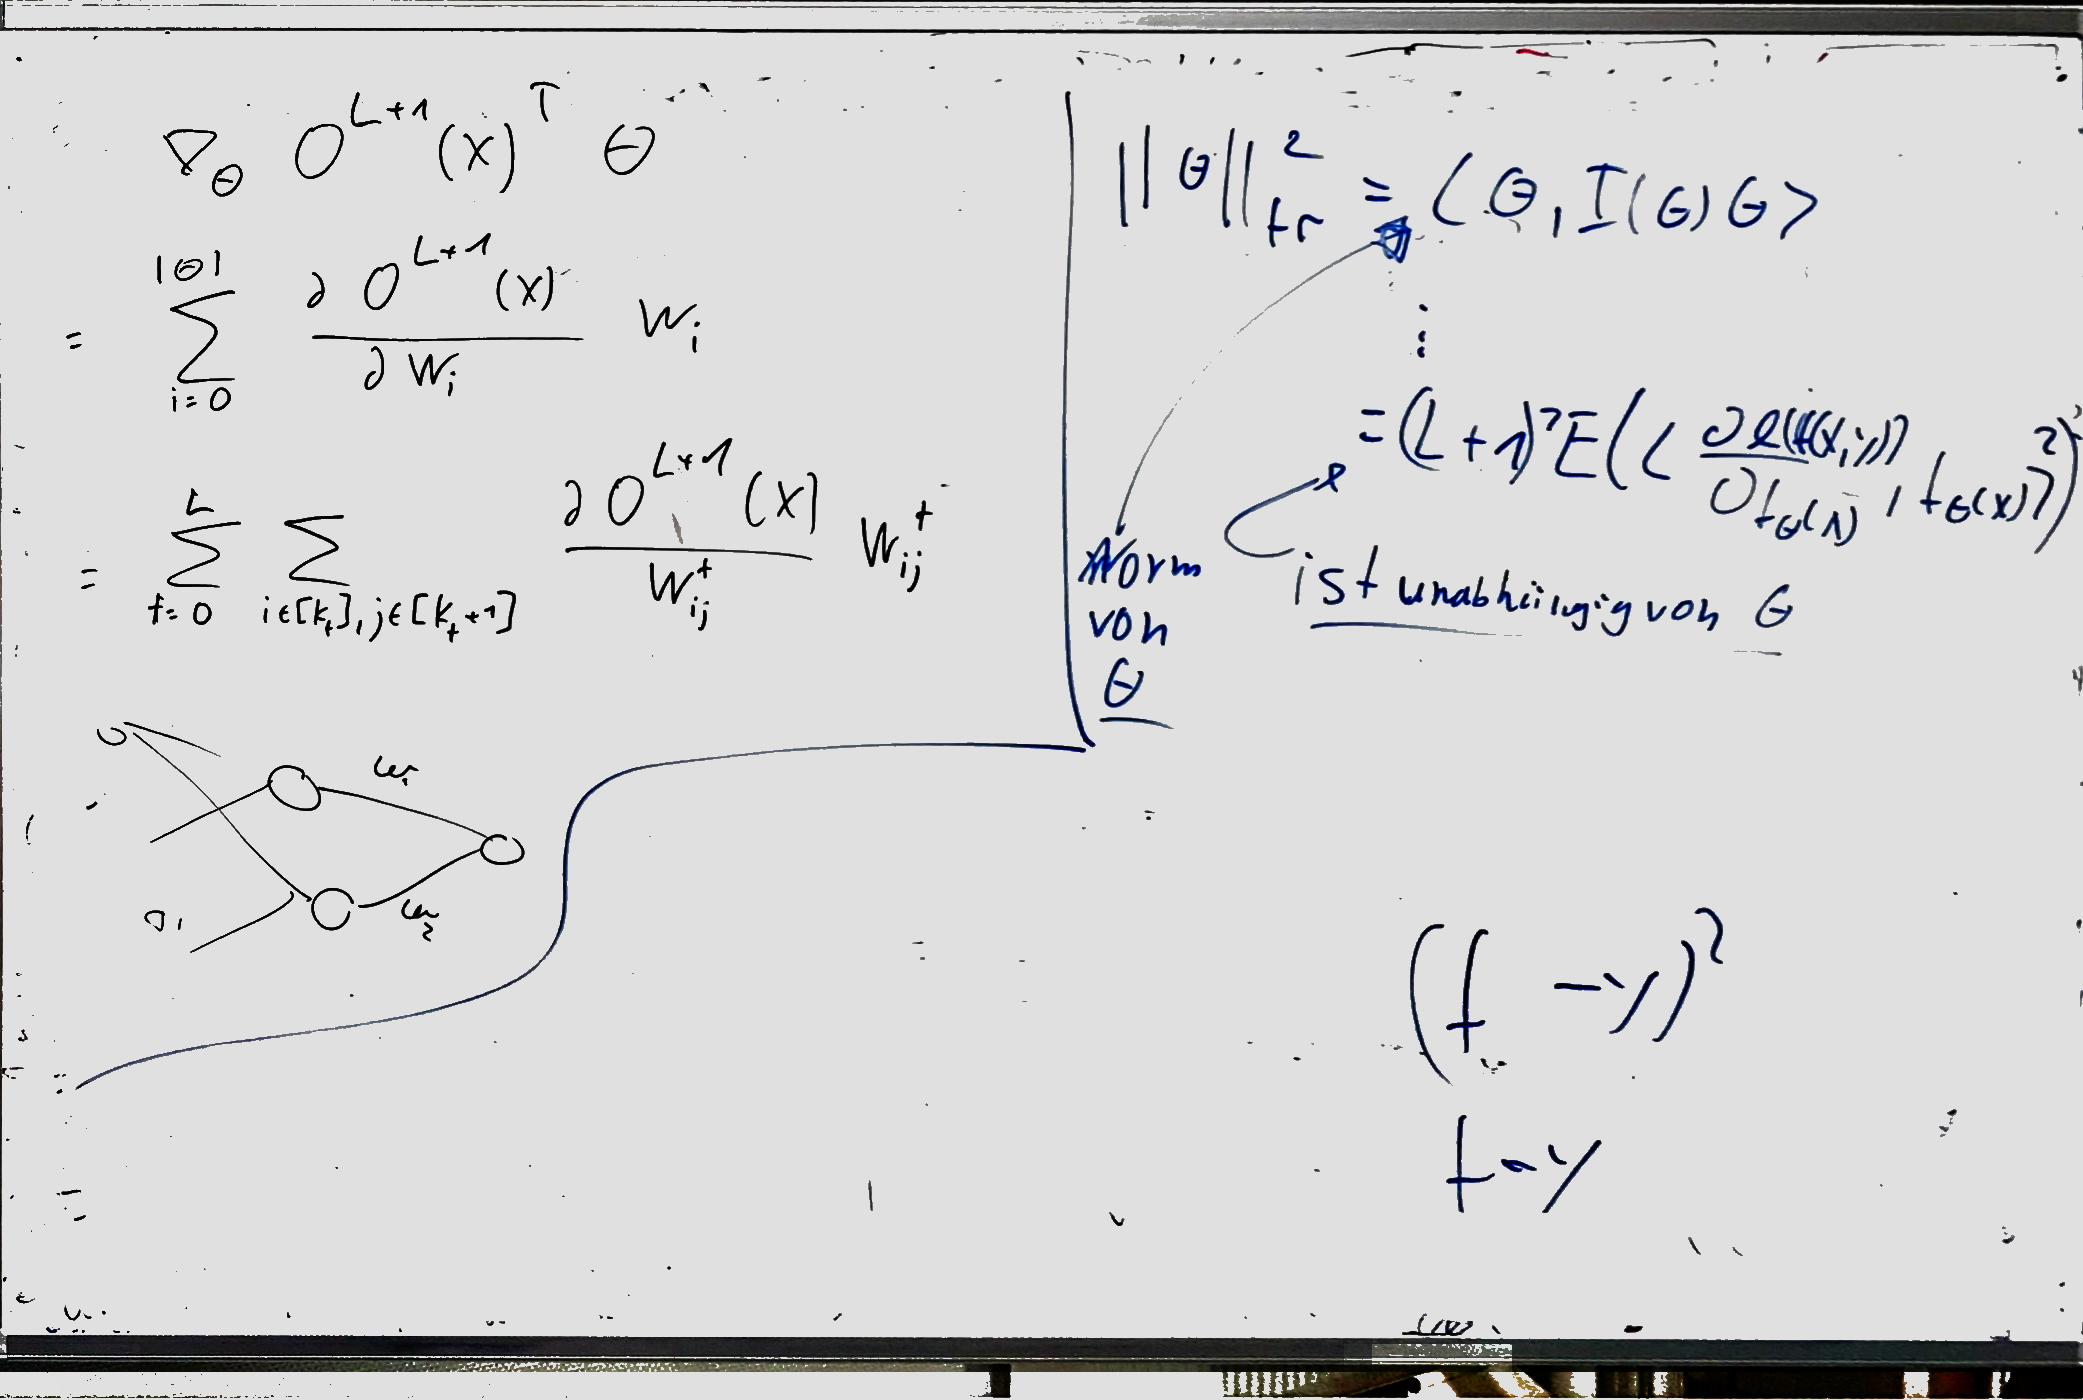
\includegraphics[width=\textwidth]{whiteboard_notes/08.jpg}
\end{figure}

\begin{figure}
	\centering
	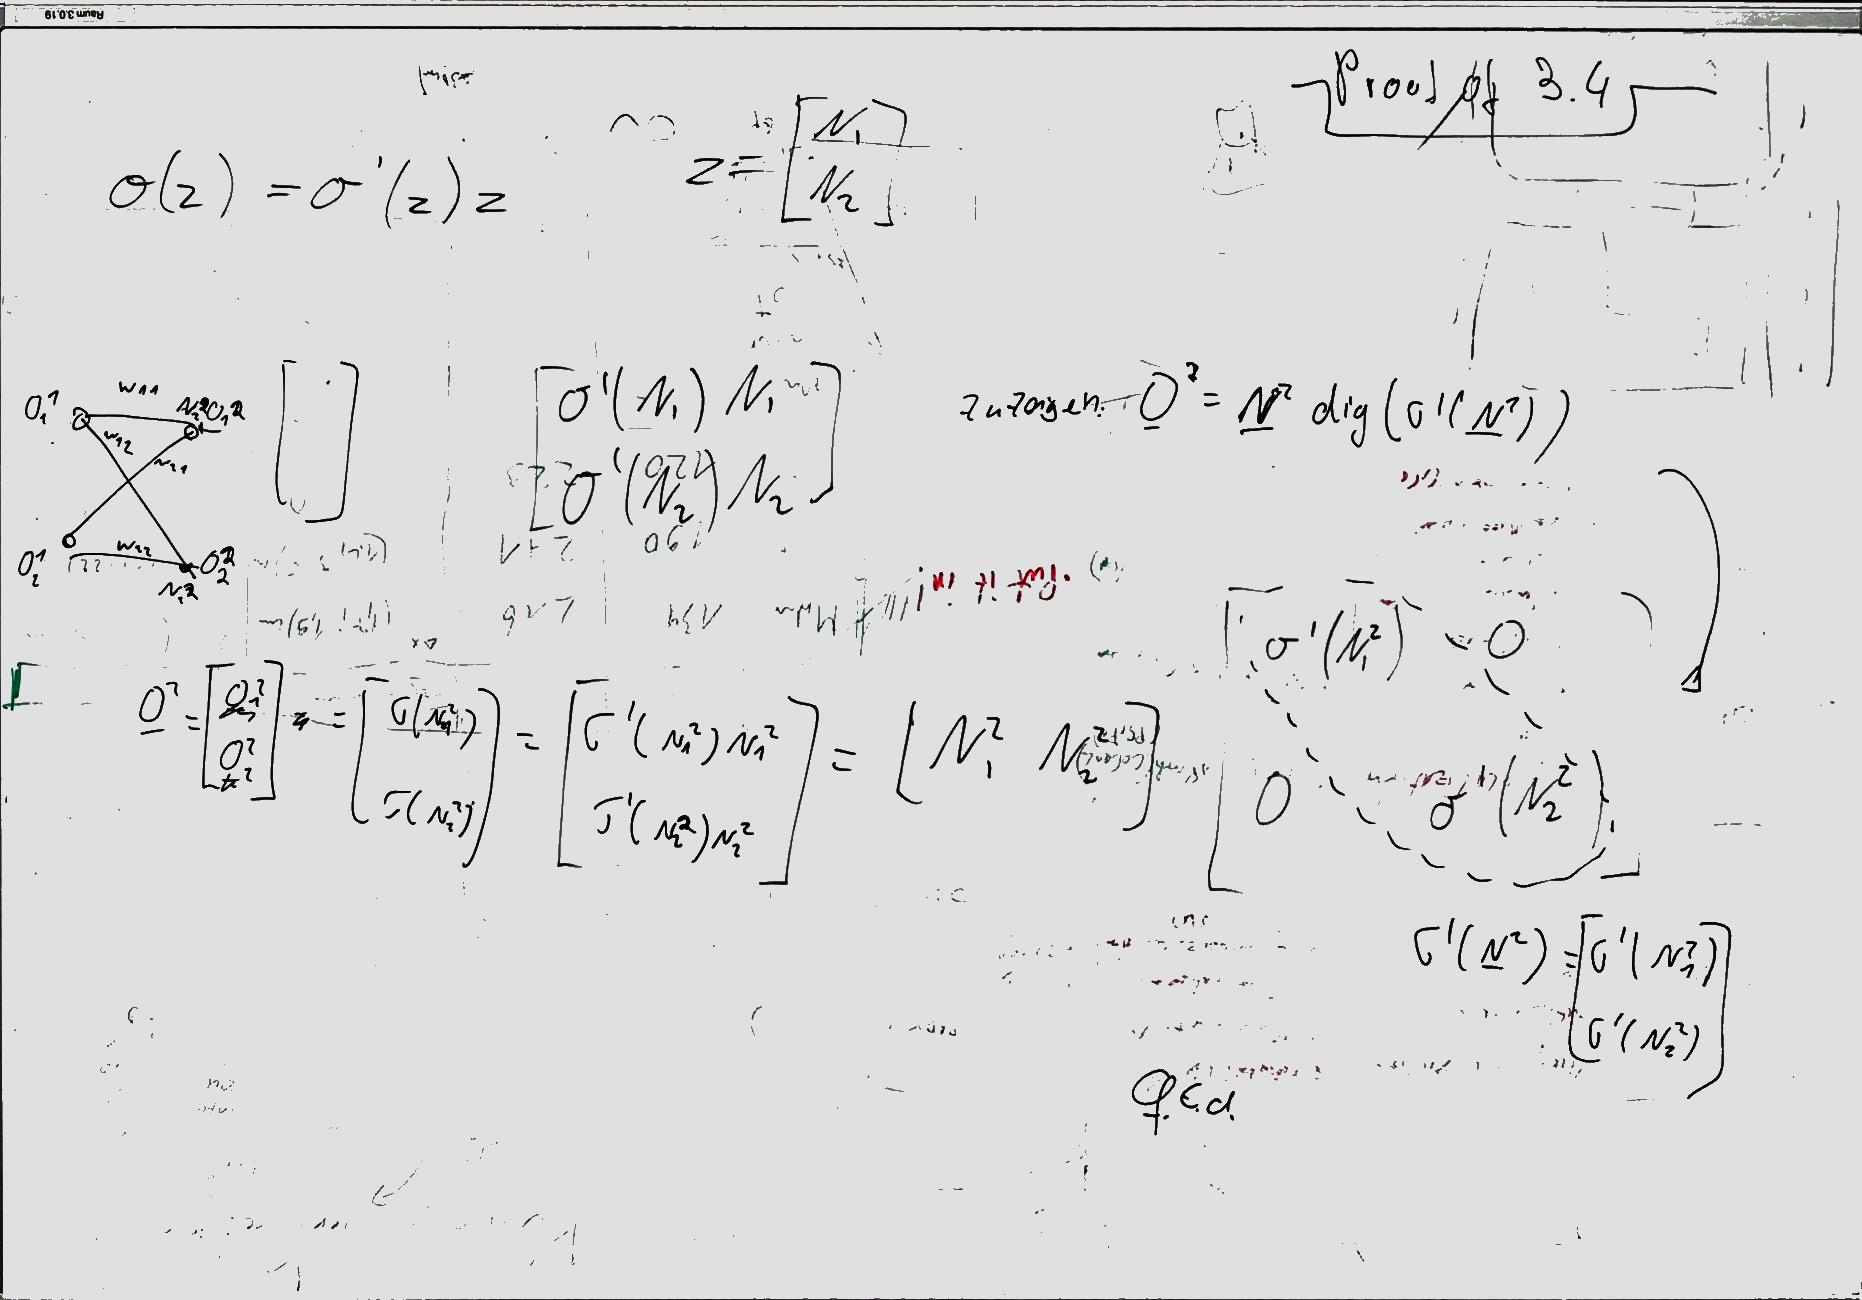
\includegraphics[width=\textwidth]{whiteboard_notes/09.jpg}
\end{figure}

\begin{figure}
	\centering
	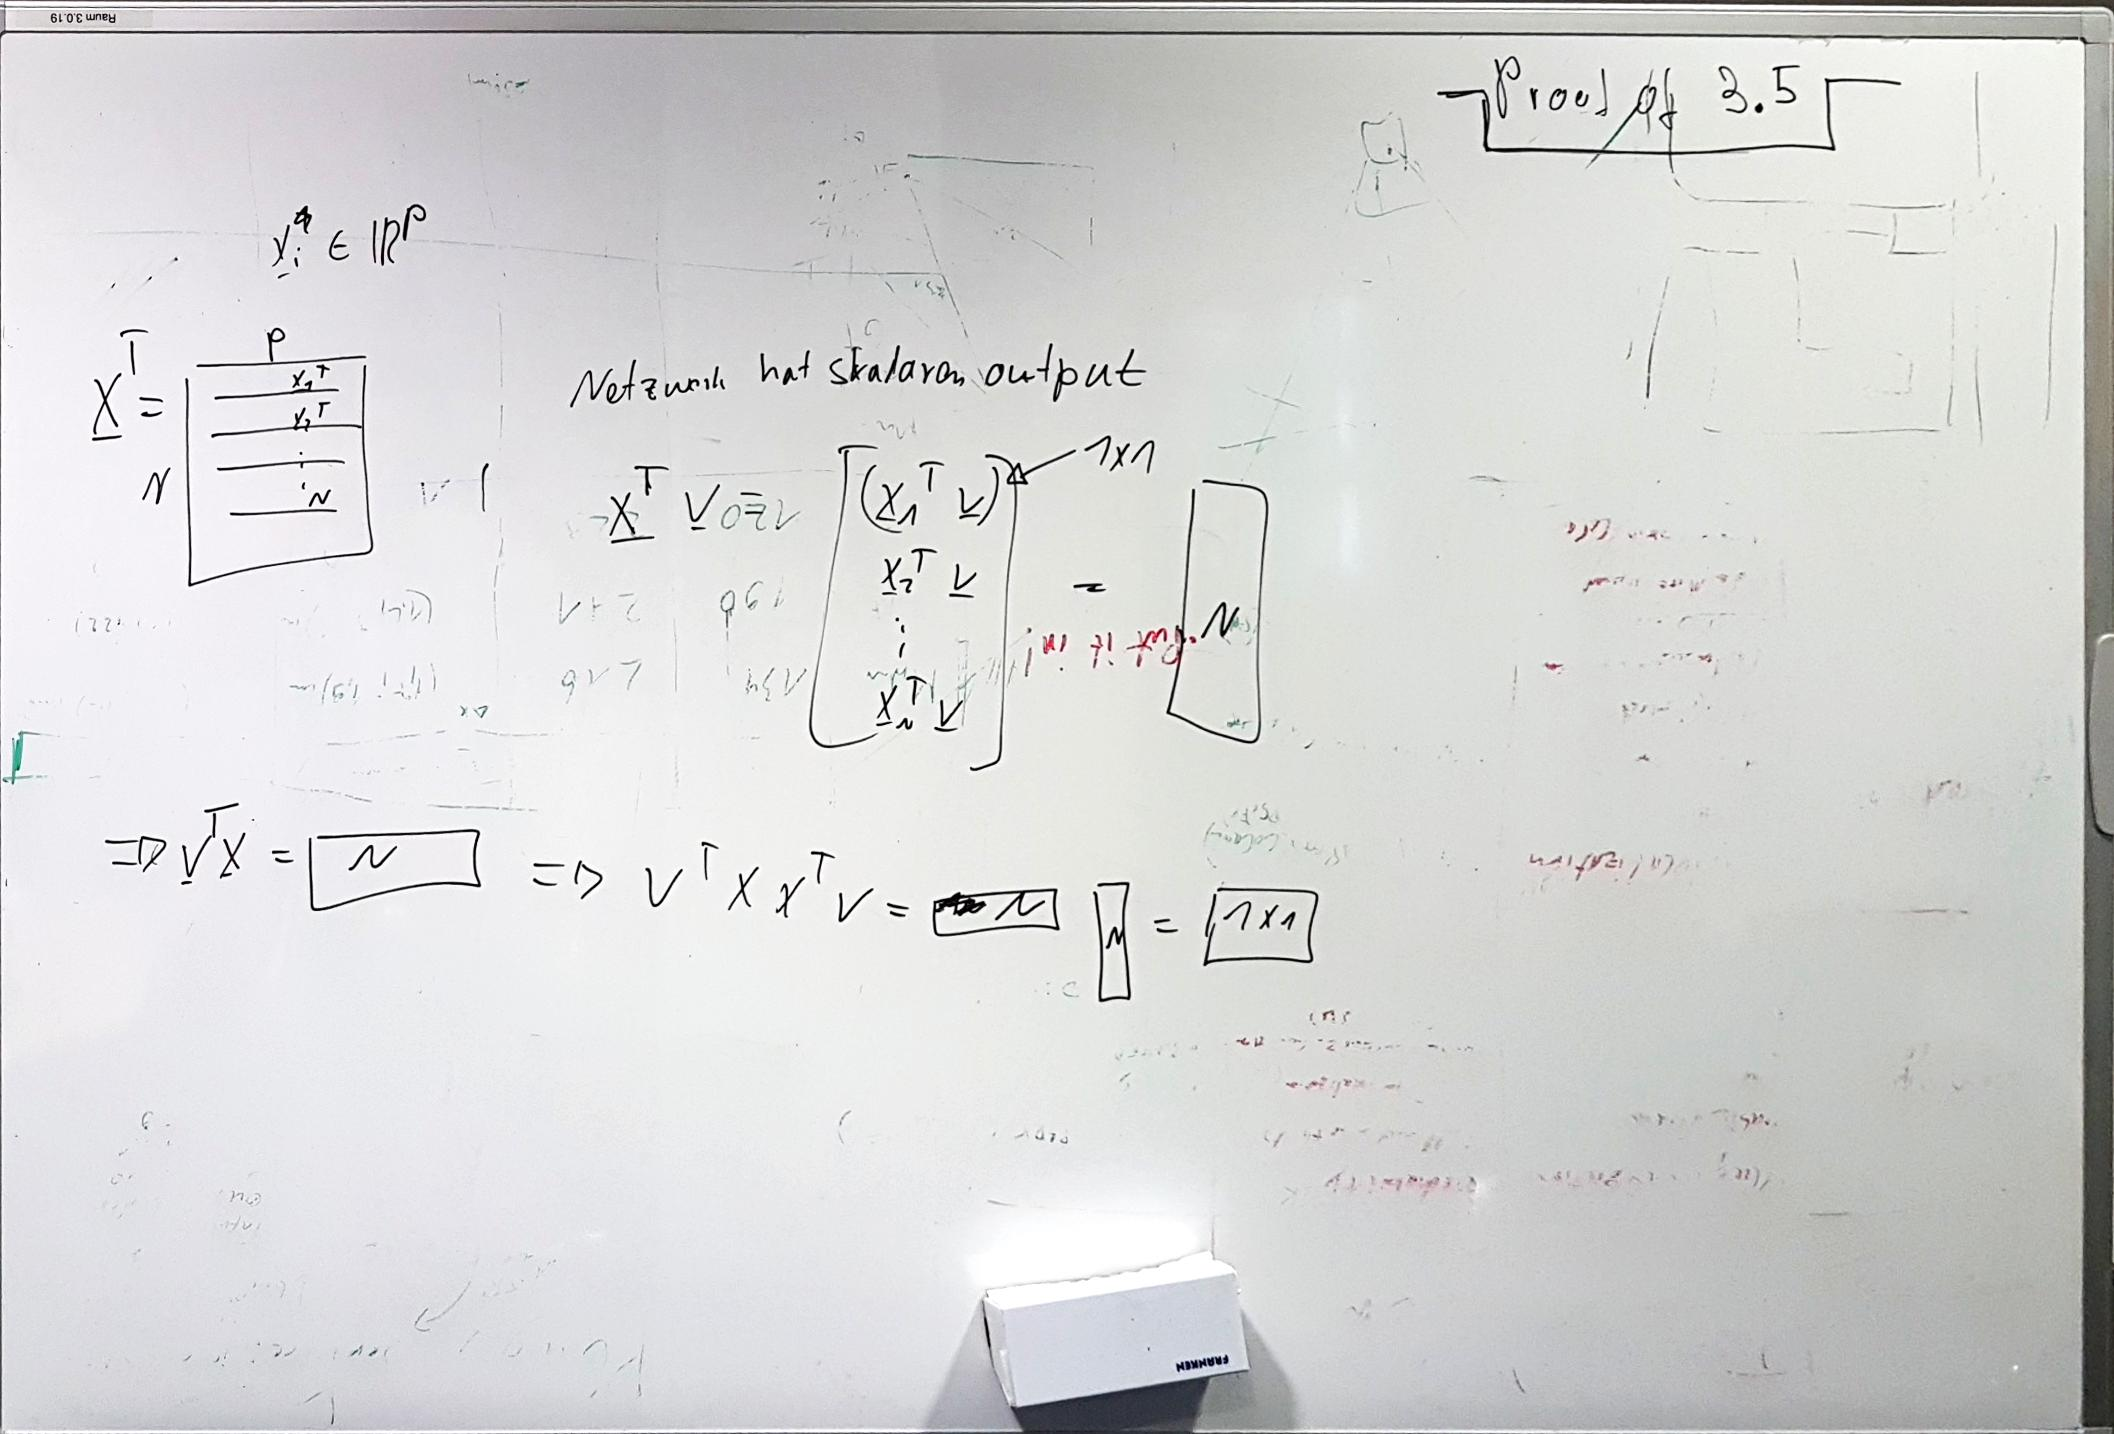
\includegraphics[width=\textwidth]{whiteboard_notes/10.jpg}
\end{figure}

\begin{figure}
	\centering
	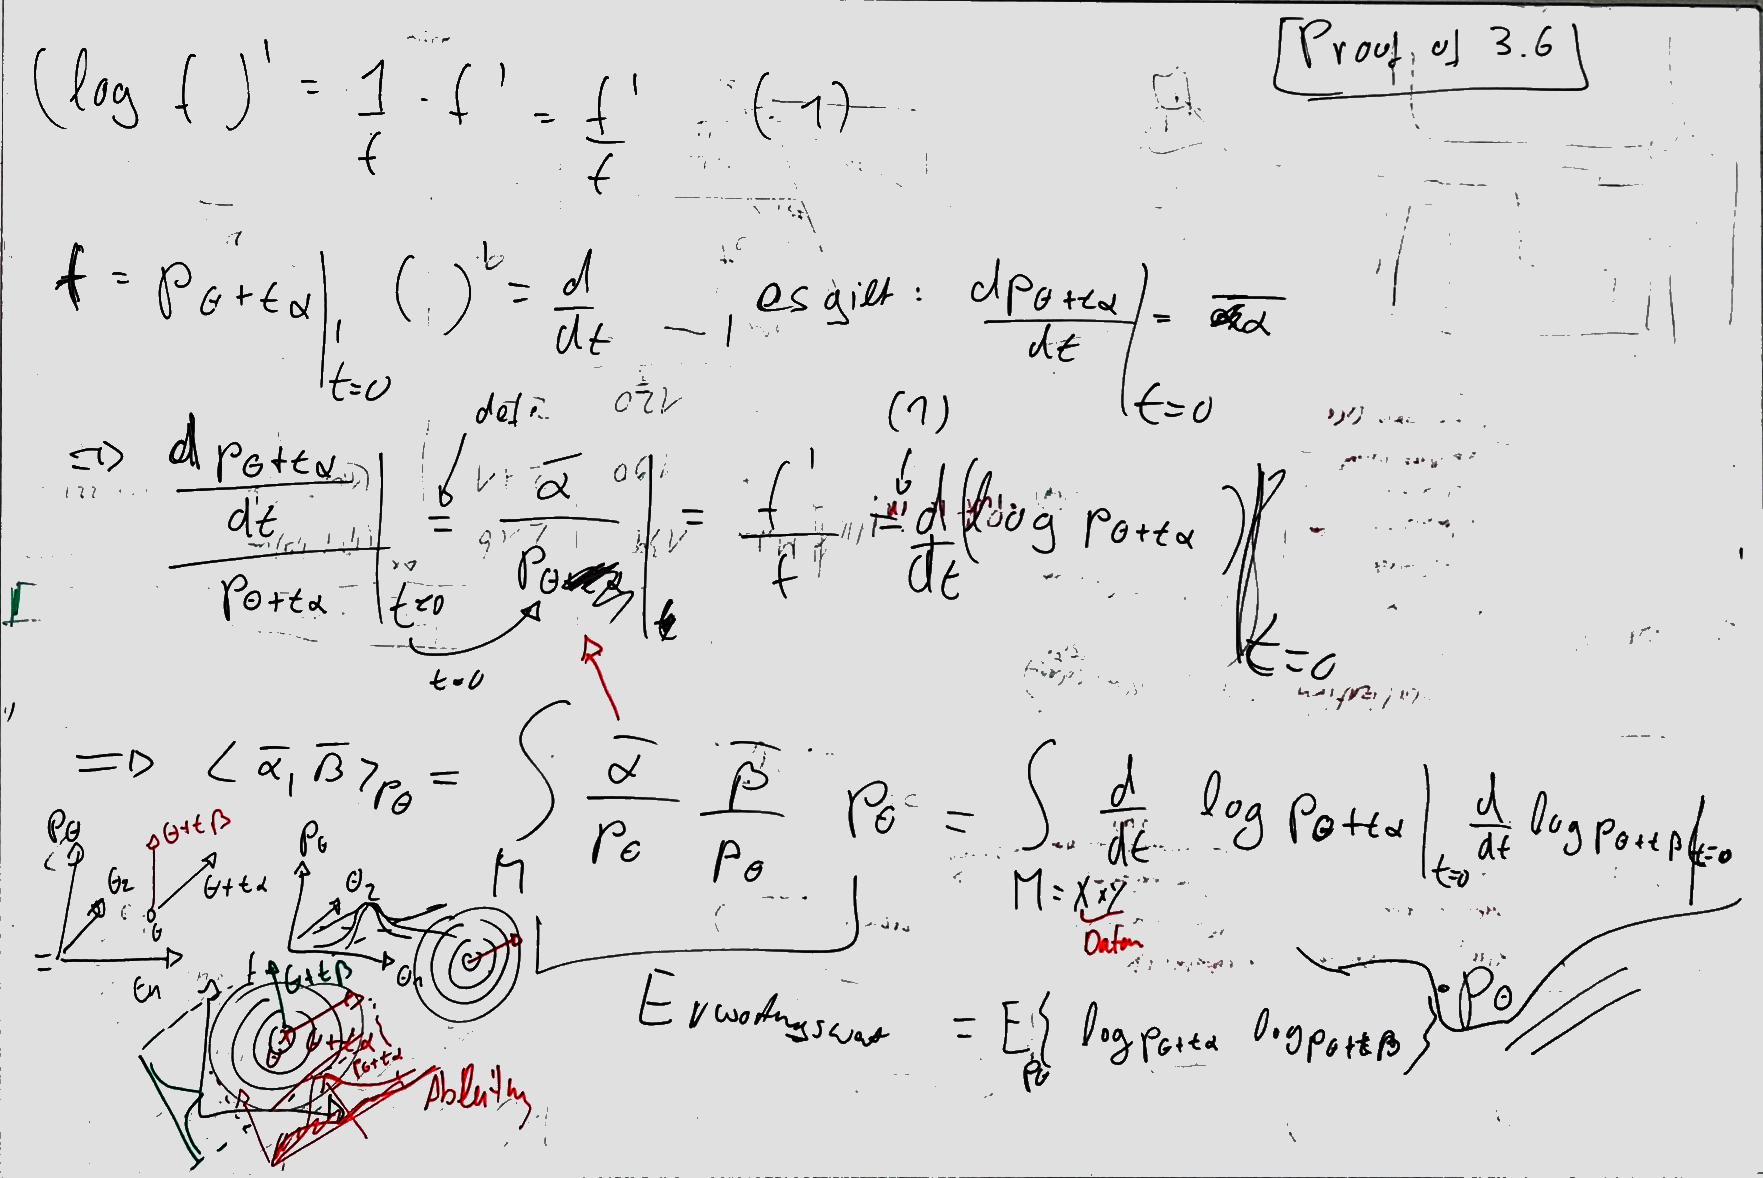
\includegraphics[width=\textwidth]{whiteboard_notes/11.jpg}
\end{figure}

\begin{figure}
	\centering
	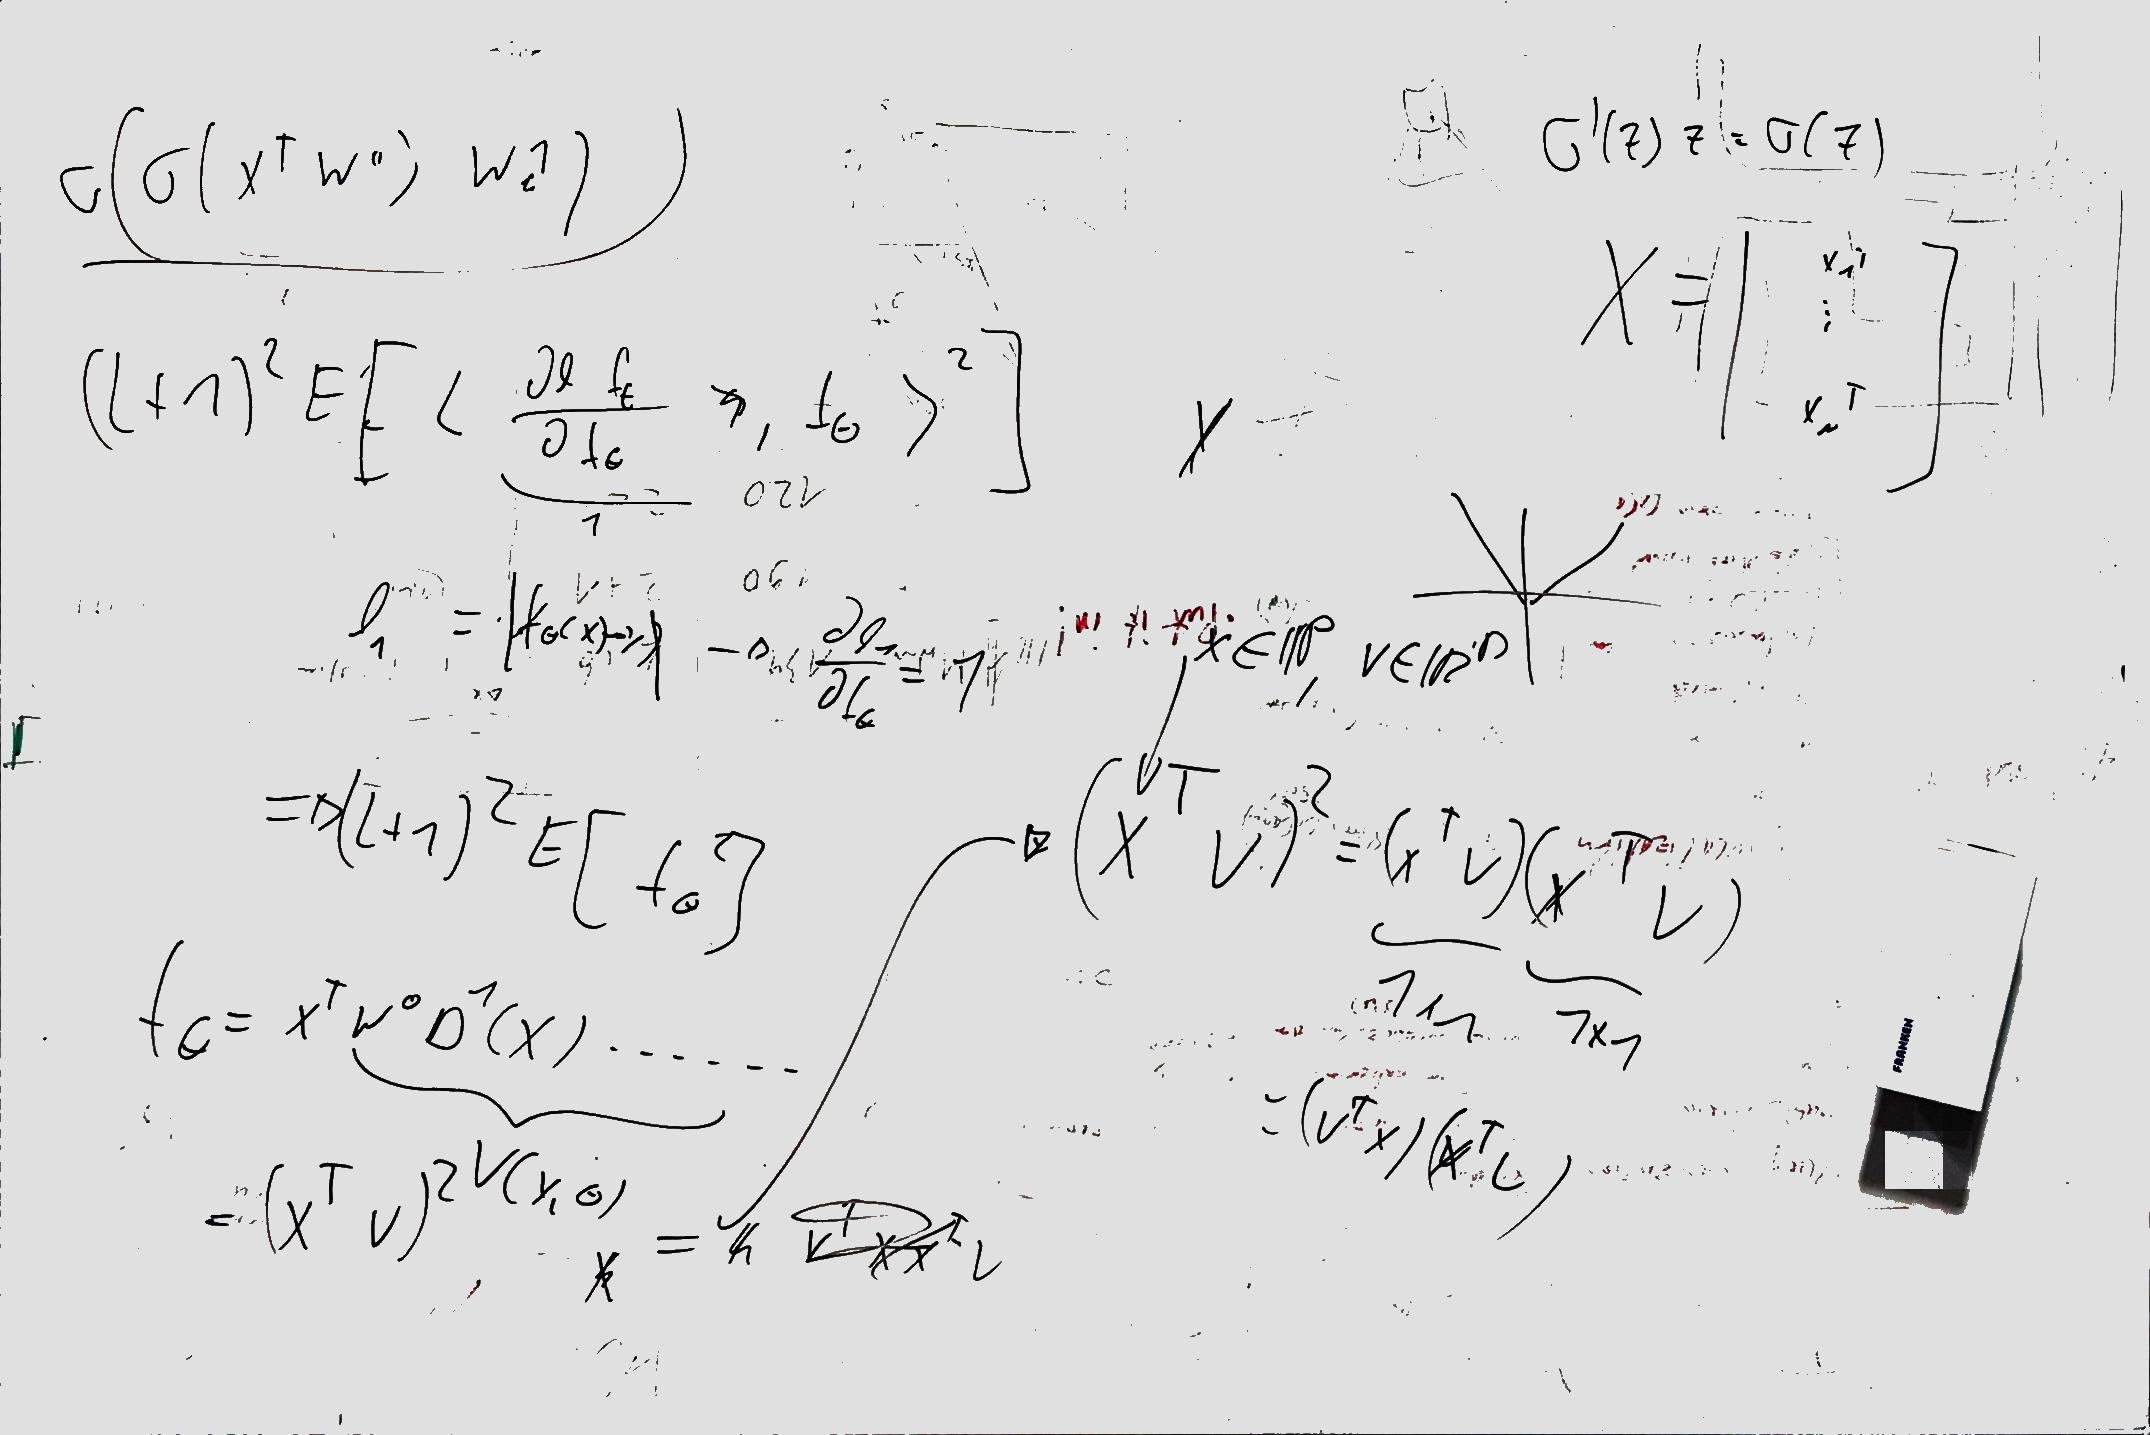
\includegraphics[width=\textwidth]{whiteboard_notes/12.jpg}
\end{figure}

\begin{figure}
	\centering
	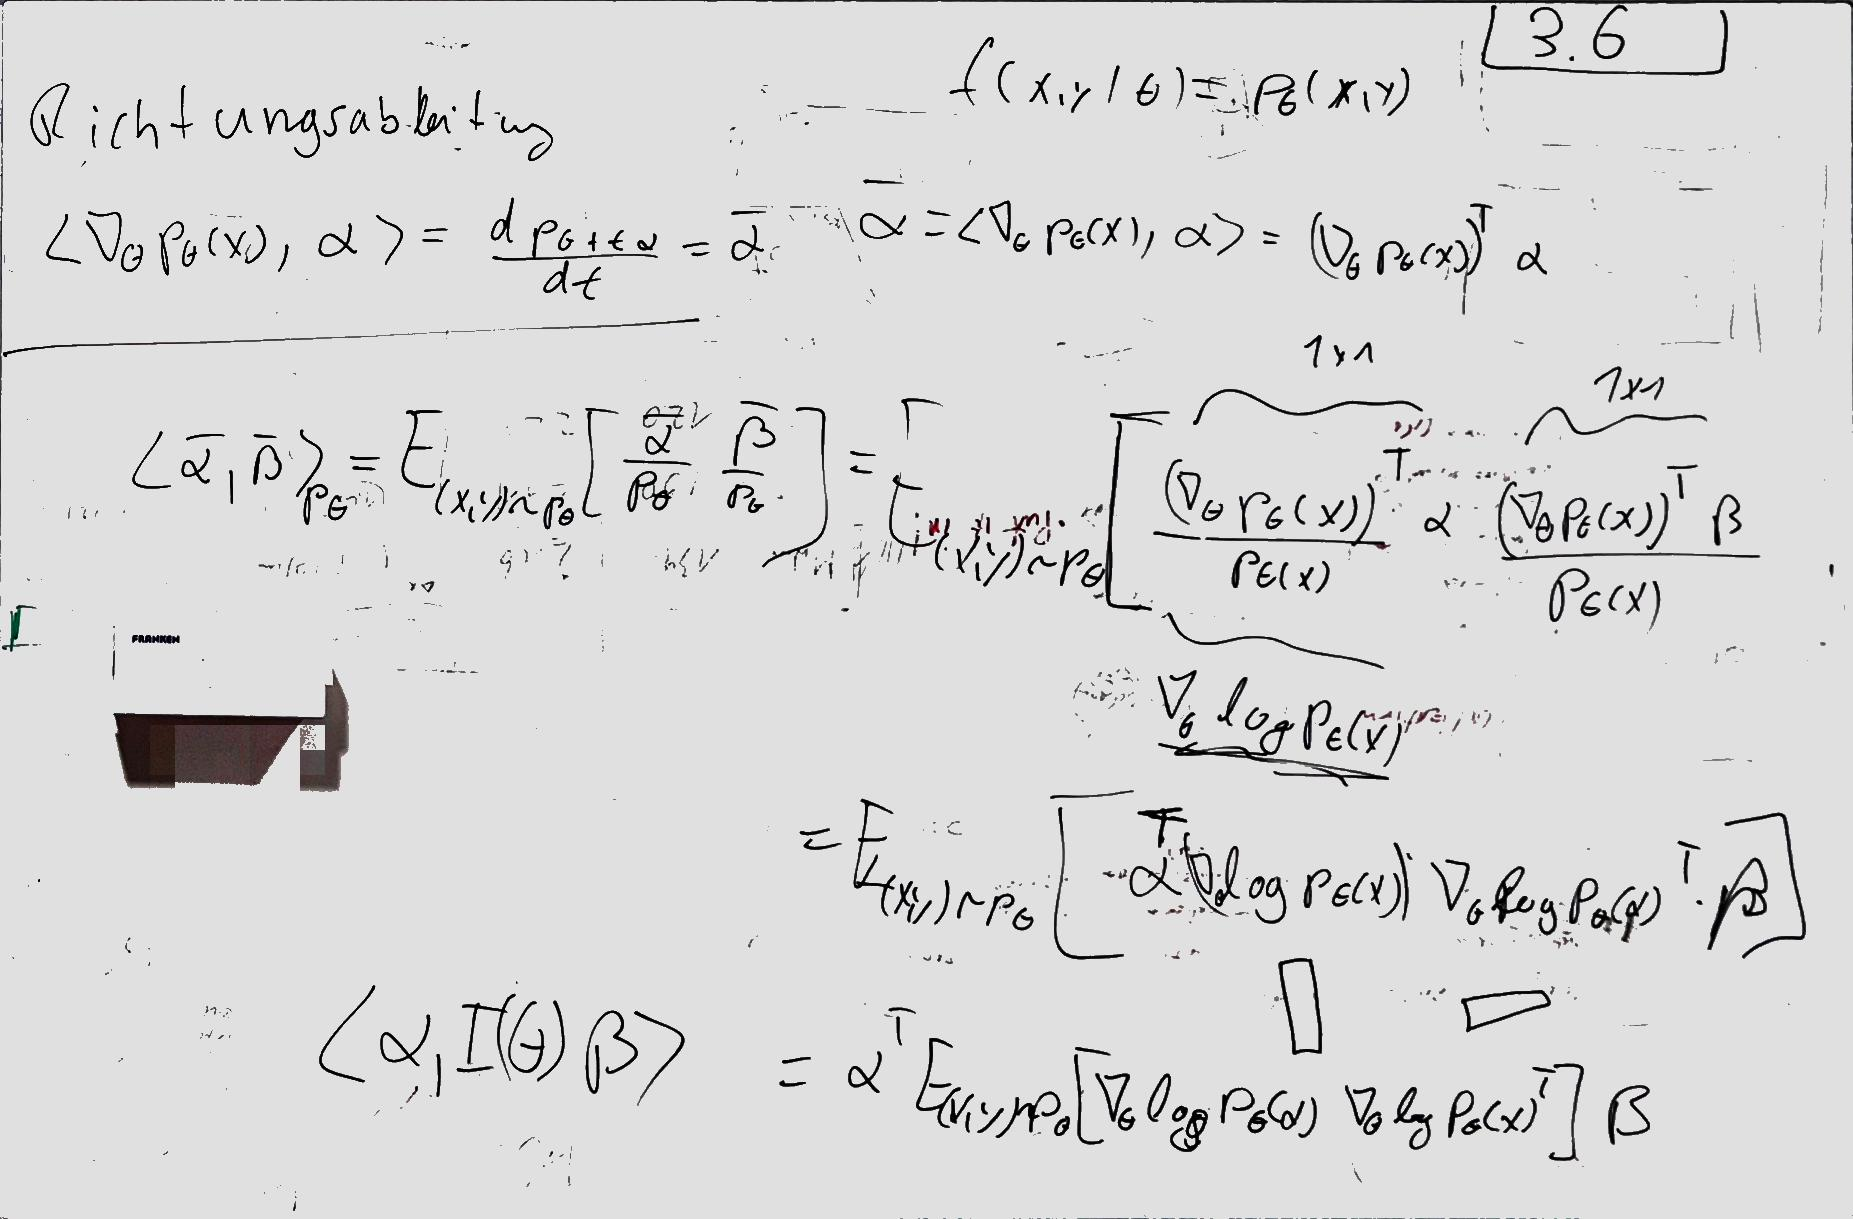
\includegraphics[width=\textwidth]{whiteboard_notes/13.jpg}
\end{figure}

\begin{figure}
	\centering
	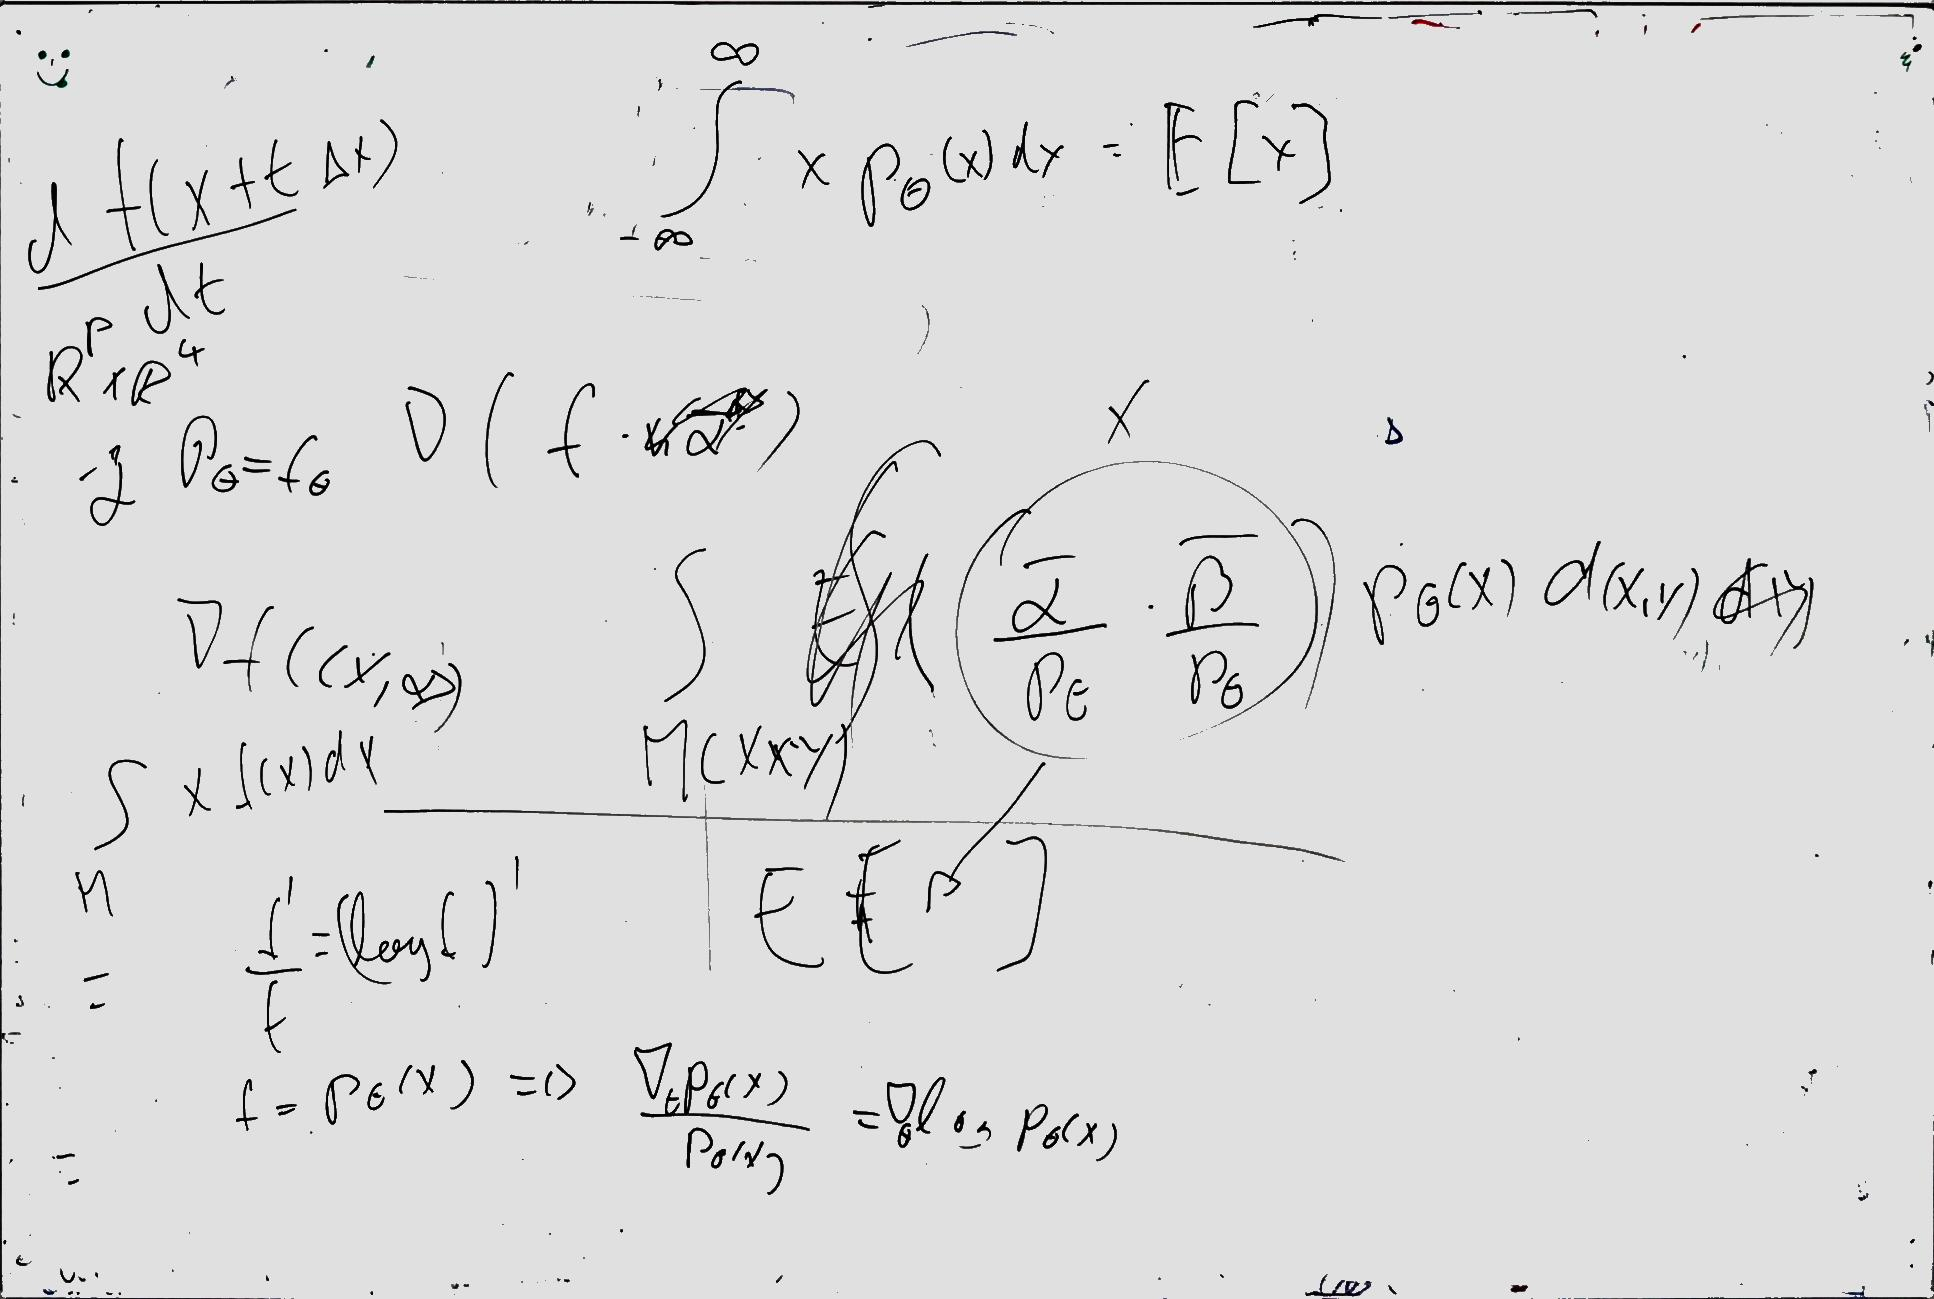
\includegraphics[width=\textwidth]{whiteboard_notes/14.jpg}
\end{figure}

\bibliographystyle{alpha}
\bibliography{sample}

\end{document}